%%
%% This is file `sample-sigconf-authordraft.tex',
%% generated with the docstrip utility.
%%
%% The original source files were:
%%
%% samples.dtx  (with options: `all,proceedings,bibtex,authordraft')
%% 
%% IMPORTANT NOTICE:
%% 
%% For the copyright see the source file.
%% 
%% Any modified versions of this file must be renamed
%% with new filenames distinct from sample-sigconf-authordraft.tex.
%% 
%% For distribution of the original source see the terms
%% for copying and modification in the file samples.dtx.
%% 
%% This generated file may be distributed as long as the
%% original source files, as listed above, are part of the
%% same distribution. (The sources need not necessarily be
%% in the same archive or directory.)
%%
%%
%% Commands for TeXCount
%TC:macro \cite [option:text,text]
%TC:macro \citep [option:text,text]
%TC:macro \citet [option:text,text]
%TC:envir table 0 1
%TC:envir table* 0 1
%TC:envir tabular [ignore] word
%TC:envir displaymath 0 word
%TC:envir math 0 word
%TC:envir comment 0 0
%%
%%
%% The first command in your LaTeX source must be the \documentclass
%% command.
%%
%% For submission and review of your manuscript please change the
%% command to \documentclass[manuscript, screen, review]{acmart}.
%%
%% When submitting camera ready or to TAPS, please change the command
%% to \documentclass[sigconf]{acmart} or whichever template is required
%% for your publication.
%%
%%
\documentclass[sigconf]{acmart}
\usepackage{hyperref}
\usepackage{enumitem}
\usepackage{pifont}
\usepackage{array}
\newlist{arrowlist}{itemize}{1}
\setlist[arrowlist]{label=$\Rightarrow$}
%%\usepackage{indentfirst}

%%
%% \BibTeX command to typeset BibTeX logo in the docs
\AtBeginDocument{%
  \providecommand\BibTeX{{%
    Bib\TeX}}}

%% Rights management information.  This information is sent to you
%% when you complete the rights form.  These commands have SAMPLE
%% values in them; it is your responsibility as an author to replace
%% the commands and values with those provided to you when you
%% complete the rights form.
\setcopyright{acmlicensed}
\copyrightyear{2024}
\acmYear{2024}
\acmDOI{}

%% These commands are for a PROCEEDINGS abstract or paper.
\acmConference[G51]{PRI}{October 13, 2024}{Porto, PT}
%%
%%  Uncomment \acmBooktitle if the title of the proceedings is different
%%  from ``Proceedings of ...''!
%%
%%\acmBooktitle{Woodstock '18: ACM Symposium on Neural Gaze Detection,
%%  June 03--05, 2018, Woodstock, NY}
\acmISBN{978-1-4503-XXXX-X/18/06}


%%
%% Submission ID.
%% Use this when submitting an article to a sponsored event. You'll
%% receive a unique submission ID from the organizers
%% of the event, and this ID should be used as the parameter to this command.
%%\acmSubmissionID{123-A56-BU3}

%%
%% For managing citations, it is recommended to use bibliography
%% files in BibTeX format.
%%
%% You can then either use BibTeX with the ACM-Reference-Format style,
%% or BibLaTeX with the acmnumeric or acmauthoryear sytles, that include
%% support for advanced citation of software artefact from the
%% biblatex-software package, also separately available on CTAN.
%%
%% Look at the sample-*-biblatex.tex files for templates showcasing
%% the biblatex styles.
%%

%%
%% The majority of ACM publications use numbered citations and
%% references.  The command \citestyle{authoryear} switches to the
%% "author year" style.
%%
%% If you are preparing content for an event
%% sponsored by ACM SIGGRAPH, you must use the "author year" style of
%% citations and references.
%% Uncommenting
%% the next command will enable that style.
%%\citestyle{acmauthoryear}


%%
%% end of the preamble, start of the body of the document source.
\begin{document}

%%
%% The "title" command has an optional parameter,
%% allowing the author to define a "short title" to be used in page headers.
\title{PRIMED: A Medicine Search System}

%%
%% The "author" command and its associated commands are used to define
%% the authors and their affiliations.
%% Of note is the shared affiliation of the first two authors, and the
%% "authornote" and "authornotemark" commands
%% used to denote shared contribution to the research.
\author{Pedro Simões}
\email{up202403063@up.pt}
\affiliation{%
  \institution{Faculdade de Engenharia da Universidade do Porto}
  \city{Porto}
  \country{Portugal}
}

\author{Miguel Garrido}
\email{up202108889@up.pt}
\affiliation{%
	\institution{Faculdade de Engenharia da Universidade do Porto}
	\city{Porto}
	\country{Portugal}
}

\author{Emanuel Maia}
\email{up202107486@up.pt}
\affiliation{%
	\institution{Faculdade de Engenharia da Universidade do Porto}
	\city{Porto}
	\country{Portugal}
}

\author{Guilherme Martins}
\email{up202403106@up.pt}
\affiliation{%
	\institution{Faculdade de Engenharia da Universidade do Porto}
	\city{Porto}
	\country{Portugal}
}

%%
%% By default, the full list of authors will be used in the page
%% headers. Often, this list is too long, and will overlap
%% other information printed in the page headers. This command allows
%% the author to define a more concise list
%% of authors' names for this purpose.
\renewcommand{\shortauthors}{Pedro Simões, Miguel Garrido, Emanuel Maia and Guilherme Martins}

%%
%% The abstract is a short summary of the work to be presented in the
%% article.
\begin{abstract}
The \textit{\textbf{PRIMED}} project aims to enhance access to structured pharmaceutical data for healthcare and research by collecting and processing information on medicines, diseases, manufacturers, and user reviews. This paper details the latest milestone, which involves data collection from diverse sources such as Kaggle and Wikipedia, followed by a comprehensive data pipeline implemented in \texttt{Python}. Key steps in this pipeline include data cleaning, text normalization, and standardization of formats, ensuring the data is structured and easily searchable. The model stores data in a \texttt{JSON} format, making it compatible with future integration into larger systems. Preliminary results indicate that the processed data improves accessibility and organization, providing a valuable resource for healthcare professionals and researchers in making informed decisions. \end{abstract}

%%
%% The code below is generated by the tool at http://dl.acm.org/ccs.cfm.
%% Please copy and paste the code instead of the example below.
%%
\begin{CCSXML}
<ccs2012>
   <concept>
       <concept_id>10002951.10003317.10003325</concept_id>
       <concept_desc>Information systems~Information retrieval query processing</concept_desc>
       <concept_significance>100</concept_significance>
       </concept>
 </ccs2012>
\end{CCSXML}

\ccsdesc[100]{Information systems~Information retrieval query processing}

%%
%% Keywords. The author(s) should pick words that accurately describe
%% the work being presented. Separate the keywords with commas.
\keywords{Medicine, Treatments, Sickness, Pipeline, Data, Gathering, Scraping, Preparation, Search Engine}
%% A "teaser" image appears between the author and affiliation
%% information and the body of the document, and typically spans the
%% page.

%%
%% This command processes the author and affiliation and title
%% information and builds the first part of the formatted document.
\maketitle

\section{Introduction}

Nowadays, accurate and comprehensive medicine information plays a vital role in decision-making on the healthcare and investigation sectors. Having access to clean and relevant information is crucial to enhance the efficiency and safety of treatments.

The \textit{\textbf{PRIMED}} project aims to compile and organize such data so that it can be accessed in an easy and organized way. It provides insights that can be applied both in practical cases or simply in developing new health safety politics.

In this part of the project, data from various sources was collected, processed and analysed with the goal of creating a solid basis for a pharmaceutical system. The whole process is described in this document, from the choice of the theme itself up to the analysis of gathered data and its subsequent classification.

\section{Theme Selection}

The choice to focus on medicines as the central theme for this project stems from the critical role they play in modern healthcare. Medication is the primary tool for treating multiple health problems and conditions, making them an essential component in both public healthcare systems and individual patient care. The data surrounding these substances, such as active substances, applicable cases and clinical trials, offers valuable insights that can improve decision-making in medical practice and pharmaceutics.

\section{Data Collection}

This chapter outlines the data selection process and the methods utilized to gather it.

\subsection{Selection of Data}

One of the main challenges of the healthcare sector is ensuring that accurate and up-to-date information on medication is available to healthcare professionals. Given these needs, the selection of data to be collected was made:

\begin{itemize}
	\item {\texttt{Medicines}}: The main component of the data, consisting of medicines and their respective relevant, intrinsic information.
	\item {\texttt{Diseases}}: To complement the collected data, information on some diseases was collected so that it would be possible to get more information to allow for an easier medicine selection process.
	\item {\texttt{Pharmaceutical Companies}}: Some pharmaceutical companies are more trusted than others due to their credibility and higher quality products, which can impact the decision-making process.
	\item {\texttt{Reviews}}: It is important to know the success rate of the presented medicine and how the people who use it feel about it.
\end{itemize}

With this data, the aim is to provide the required information to the users.

\subsection{Gathering}

Finding data suitable for the project proved to be a challenge; not only did it have to be relevant and accurate, but it also had to meet some criteria in terms of quantity and quality. Therefore, the data had to be gathered from multiple sources using different methods - most of the data came from prepared datasets found on Kaggle\cite{kaggle}, while the rest came from scraping Wikipedia\cite{wikipedia}.

\subsubsection{Medicines}

The \textit{Medicines} dataset\cite{medicines_dataset}, retrieved from Kaggle, contains a list of pharmaceutical treatments and some relevant, mostly textual, information about the cases where it is used.

The present information on this dataset is:
\begin{itemize}
	\item {\texttt{Medicine Name}}: The name of the medicine.
	\item {\texttt{Composition}}: The active substance present in the medicine.
	\item {\texttt{Uses}}: A list of cases where the medicine is used (specific diseases, for example).
	\item {\texttt{Side Effects}}: Lists possible side effects resulting from the medicine's usage.
	\item {\texttt{Manufacturer}}: The name of the company responsible for producing the medicine.
	\item {\texttt{Reviews}}: Three additional columns containing the percentage of "Excellent", "Average" and "Poor" reviews for each medicine's treatment results.
\end{itemize}

This dataset, which contains 11824 different medicines, possesses a {\textit{\textbf{CC0 1.0 Universal}}}\cite{cczero} license, which means the data is part of the public domain, allowing for the copying and modification of the data.

\subsubsection{Diseases}

This dataset was scraped from the tables of a Wikipedia page containing a list of autoimmune diseases\cite{diseases_dataset}; by gathering this data, the goal was to complement the previous dataset's "Uses" and "Side Effects" columns by collecting more information on this specific subset of diseases.

The information extracted from this dataset consists of:
\begin{itemize}
        \item {\texttt{Disease}}: The name of the disease.
	\item {\texttt{Primary Organ/Body Part Affected}}: Information on the organs or body parts affected by the disease.
	\item {\texttt{Autoantibodies}}: The antibodies associated with each specific disease.
	\item {\texttt{Acceptance as an Autoimmune Disease}}: Classification for each disease related to its acceptance as an autoimmune condition, based on the current scientific consensus and level of evidence supporting its autoimmune nature.
	\item {\texttt{Prevalence Rate (US)}}: The percentage of people affected by the disease in the United States of America.
\end{itemize}

The gathered dataset contains about 110 lines of diseases, being available under the \textit{\textbf{Creative Commons Attribution-ShareAlike 4.0 International}}\cite{wikipedia_cc} license, which allows for the sharing and adaptation of the contents.

\subsubsection{Pharmaceutical Companies}

To complement the data on companies present in the \textit{Medicines} dataset, more data on pharmaceutical companies was gathered through another round Wikipedia scraping - this time from a page containing an extensive list of pharmaceutical companies\cite{companies_dataset}. Approximately 700 companies' names and founding dates were gathered, alongside a short description from each one's Wikipedia article.

The collected information follows this structure:
\begin{itemize}
	\item {\texttt{Company Name}}: The company's name.
	\item {\texttt{Year}}: The year the company was created and, if available, when the company was shut down.
	\item {\texttt{Description}}: A short description of each company, its values and some extra information.
\end{itemize}

This dataset falls under the same license as the previous \textit{Diseases} dataset (\textit{\textbf{Creative Commons Attribution-ShareAlike 4.0 International}}), as the data was collected in a similar way.

\subsubsection{Reviews}

Lastly, a dataset containing reviews for the collected medication data with more personal descriptions from users\cite{reviews_dataset} was retrieved from UC Irvine's Machine Learning Repository\cite{irvine}.

The data collected had the following structure:
\begin{itemize}
	\item {\texttt{Unique ID}}: The unique identification of the review.
	\item {\texttt{Drug Name}}: Name of the drug/treatment.
	\item {\texttt{Condition}}: The condition of the patient where it was used.
	\item {\texttt{Review}}: Written review of the experience of taking the drug.
	\item {\texttt{Rating}}: Number from 0-10 that expresses the quality of the drug.
    \item {\texttt{Date}}: Date of when the drug was taken.
    \item {\texttt{Useful Count}}: Similar to a "like" system, this showcases the number of people who found this review useful.
\end{itemize}

Each review can only be associated with a single condition/disease, which is a limitation of the dataset itself.

This dataset contains around 215000 entries and is covered by the \textit{\textbf{Attribution 4.0 International}}\cite{ccfour} license, which allows for the sharing and adaptation of the datasets for any purpose, provided that the appropriate credit is given.

\section{Pipeline Description}

As mentioned in section 3.2 of this report, \textit{\textbf{PRIMED}}'s data comes from various sources. Due to the often unstructured nature of this data, it is vital to have a streamlined and automated way of normalizing and processing all the information into similar formats, which is the main role of the data pipeline, present in figure~[\ref{fig:pipeline}].

\begin{figure}[h]
	\centering
	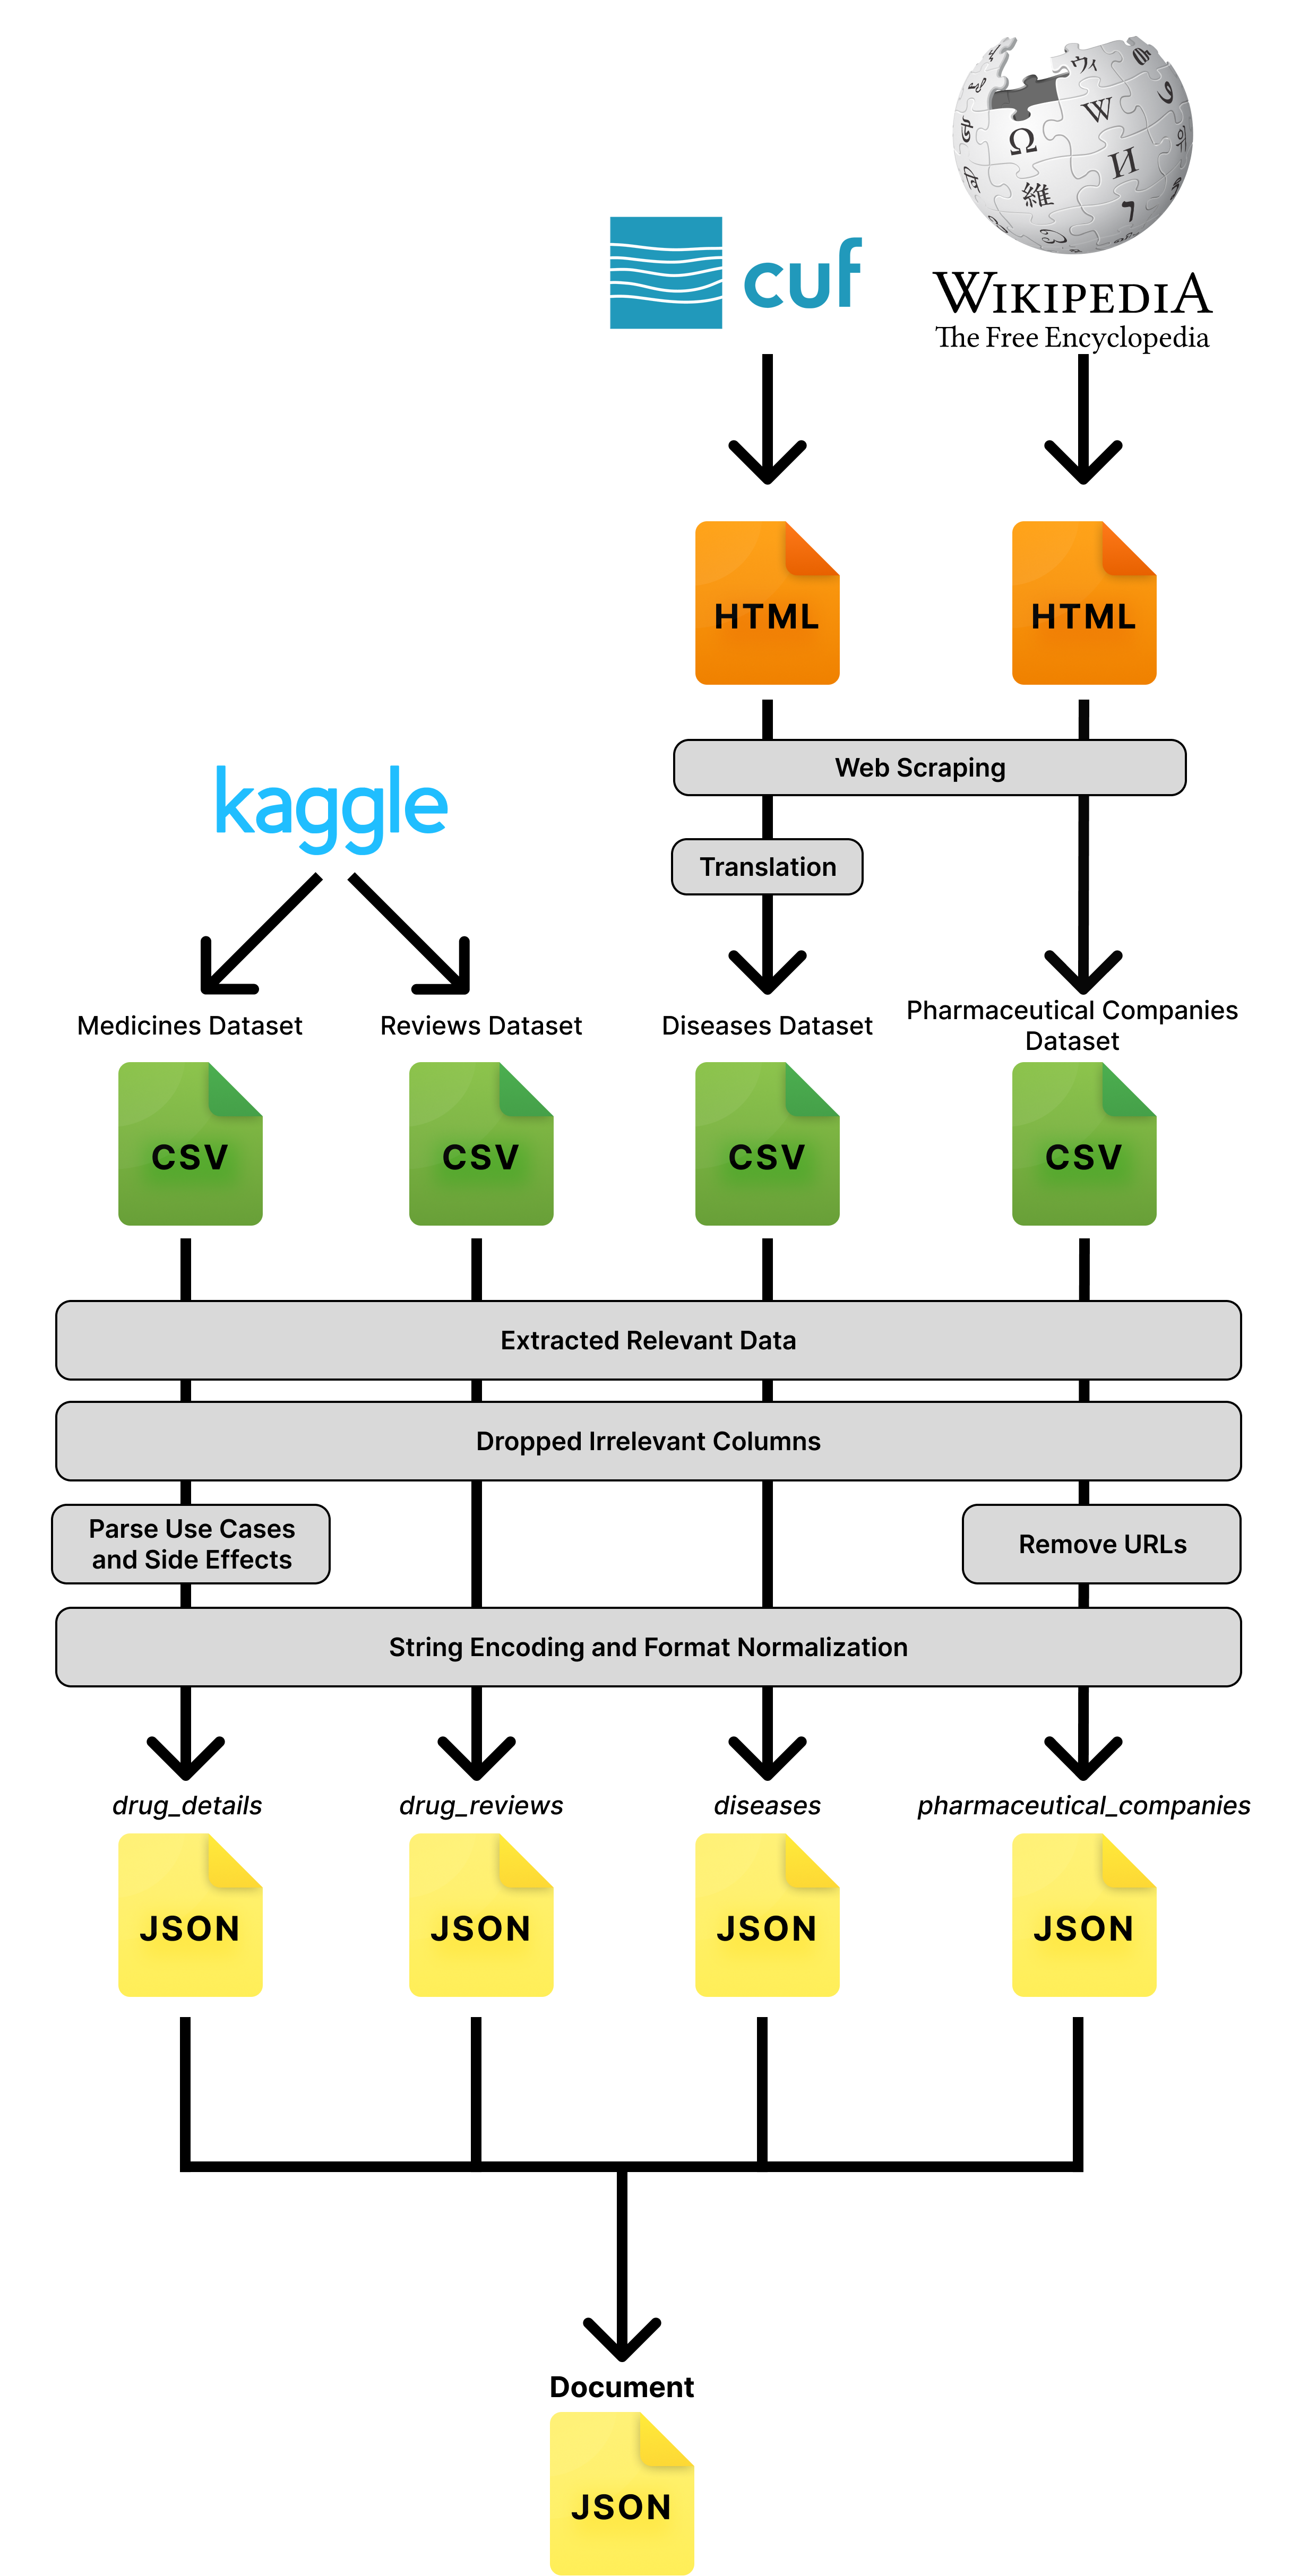
\includegraphics[width=\linewidth]{data_pipeline.png}
	\caption{Data Pipeline}
	\Description{Data Pipeline}
	\label{fig:pipeline}
  \end{figure}

The pipeline consists of \texttt{Python}\cite{python} scripts utilizing libraries such as \texttt{pandas}\cite{pandas}, \texttt{unidecode}\cite{unidecode}, \texttt{html}\cite{html}, \texttt{json}\cite{json} and \texttt{csv}\cite{csv} with the crux of the data processing occurring on the \texttt{to{\textunderscore}json.py} script, which converts the \texttt{CSV} files into \texttt{JSON} format.

\subsection{Elimination of Null Values and Rows}

When processing data, another key aspect to consider is that not all data may be correct or even present. For this reason, before doing anything else with the \texttt{CSV} source files, the pipeline uses \texttt{pandas} \textit{dataframes} to check for and remove rows containing only null values, or rows in which key values, such as \texttt{Medicine Name}, for instance, aren't present.

\subsection{Text Normalization}

When scraping information from websites, it is important to make sure all the text is normalized. The data pipeline ensures, via \texttt{Python}'s \texttt{unidecode()} function, that the dataset only contains \texttt{ASCII} characters. This helps prevent future issues when searching the datasets for information.

Another character normalization problem resulting from the scraping process arises due to \texttt{HTML}'s nature - more specifically, escape codes used to represent special characters. To convert these codes into ASCII characters, the \texttt{unescape()}\cite{html} function from \texttt{Python}'s \texttt{html} module, wrapped inside a call to the previously mentioned \texttt{unidecode()} function, to convert the \texttt{Unicode} output into \texttt{ASCII}.

\subsection{Standardization of Formats}

For the best possible result, formats such as dates should be standardized; therefore, part of the pipeline deals with transforming this data into \texttt{yyyy-mm-dd} format, which makes the process of sorting and searching substantially easier. 

\subsection{Data Storage}

The final output of the pipeline (the processed data that the search engine will be working with) is stored in \texttt{JSON} format. This decision stems from the requirement of a document-based data storage model, where each \texttt{JSON} object represents a document encapsulating all the relevant fields and values for a particular record - in this case, a specific medicine. This approach provides flexibility in handling unstructured data, since there are no hard constraints in place.

This model also ensures the search engine can query and retrieve data efficiently, based on specific fields within these documents, ensuring that the system can scale as the dataset grows; it also supports complex data relationships and makes it easier to analyse information across different records.

\section{Conceptual Data Model}

Having finalized the data collection and the subsequent transformation and storage processes in the pipeline, a conceptual data model for the combined dataset was developed.

\begin{figure}[H]
  \centering
  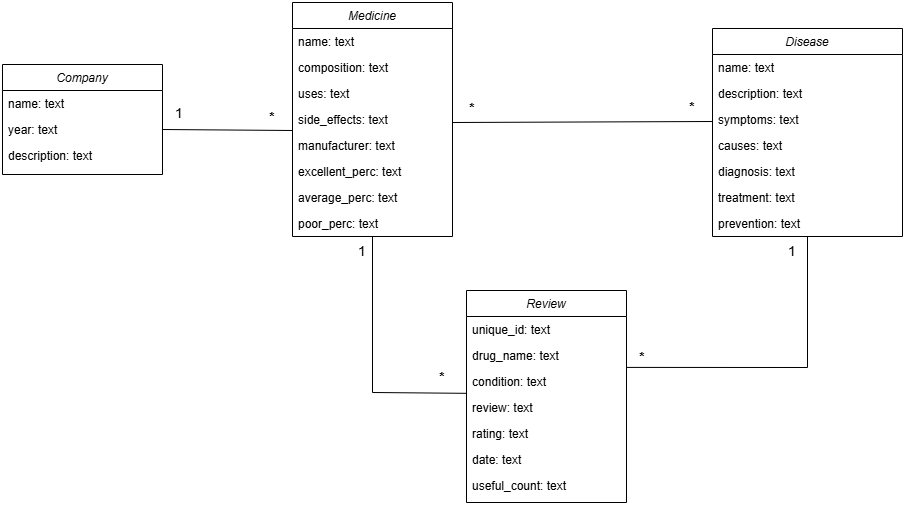
\includegraphics[width=\linewidth]{pri_uml_final.png}
  \caption{Conceptual Data Model}
  \Description{UML diagram for \textit{\textbf{PRIMED}}'s data}
  \label{fig:uml}
\end{figure}

Each medicine is associated with one and only one pharmaceutical company; a company, however, can produce multiple medicines. A single medicine can be linked to multiple diseases and reviews, though the reverse is true only for diseases - a disease can be associated to many medicines (and many reviews). A review, however, can only be associated with a single medicine and a single disease.

\section{Dataset Characterization}

With regard to the characterization of the dataset, the data resulting from the pipeline was analysed. Graphs, tables and even word clouds, despite not being the most reliable method, were created to make it easier to understand the structure of the data and the patterns that guide the system itself.

\subsection{General Description}

The final version of the dataset, representing the collection of documents, contains 11498 entries. Each entry represents a medicine along with its related information, such as associated diseases and possible side effects, user reviews, ratings and manufacturer details.

\subsection{Distribution of Drug Manufacturers}

By analysing figure~[\ref{fig:topManufacturers}], which shows the distribution of the main pharmaceutical companies responsible for manufacturing medicines where the five that possess the largest share are highlighted, we are given a clearer understanding of each manufacturers' production capabilities.

\subsection{Distribution of Reviews}

A box plot, present in figure~[\ref{fig:reviewDistribution}], is utilized to analyse the distribution of “Excellent”, “Average” and “Poor” review percentages across the different medicines. The graph shows that, for instance, "Excellent" reviews percentages are more evenly spread than the "Average" reviews percentages which, despite having a lower interquartile range\cite{iqrange}, possesses a higher number of outliers. The "Poor" review percentages have the largest variations, but also the lowest values. 

In figure~[\ref{fig:reviewPercMean}], we can see the average percentage of reviews for the top ten use cases, which supports the findings from figure~[\ref{fig:reviewDistribution}].

\subsection{Distribution of Side Effects}

By analysing figure~[\ref{fig:sideEffectsDistribution}], we can identify the most common side effects caused by medication - nausea, headaches, diarrhea - and how many medicines are associated to each one of them. As expected, the data shows that side effects that occur more frequently are those that are milder in nature.

\subsection{Common Uses Word Cloud}

Figure~[\ref{fig:commonUses}] contains a word cloud with the most common use cases for medicines. “Bacterial Infections” and "Hypertension", for example, are clearly highlighted in the graph, being conditions that are found and treated more frequently.

\subsection{Most Common Drug Compositions}

Figure~[\ref{fig:commonDrugCompositions}] identifies the the most common drug combinations available in the market, with “Levocetirizine + Montelukast” being the most prevalent, followed by other combinations such as “Luliconazole” and “Domperidone + Rabeprazole”.

\subsection{Years with the Most Companies Foundations}	

By analysing figure~[\ref{fig:companyYears}], it's possible to observe the years in which the most pharmaceutical companies were founded, with 2003 standing out. This temporal analysis gives us some information about periods of significant growth in the pharmaceutical industry.

\section{Information Needs}

The information needs can vary depending on the person using \textit{\textbf{PRIMED}}. If the individual who is using the tool is, for example, a doctor or a pharmacist, these needs might be related to the compositions of a medicine or cases where it can be applied. If the user is a patient (an average person), they might be more interested in checking which company manufactures the medicine to check if it can be trusted or to assess other user's reviews of that treatment, as well as possible side effects, to have a better understanding of what can happen to them.

Here is a list of possible information needs, explaining what type of data is needed, why and for whom:
\begin{itemize}
	\item {\texttt{Medicine Compositions}}: The composition of medication is an important aspect since some might be harmful to the patient, depending on what kind of active substances are present.
	\item {\texttt{Uses}}: Not every medicine has clearly defined use cases; some may have a primary use while also being beneficial for other less common conditions.
	\item {\texttt{Side Effects}}: The users should be aware of possible side effects resulting from their treatment, so that they can be informed and prepared for potential symptoms or strange events.
	\item {\texttt{Manufacturer}}: Some people have a preference for specific manufacturers who they trust more than others, or can simply want to gather more information on the company producing the medicine they were prescribed.
	\item {\texttt{Reviews}}: For all possible types of users, existing reviews are always important - whether they are textual or not. These indicate other people's experiences with a particular medicine and can even report some peculiar cases where the patients experienced rare effects from that treatment.
	\item {\texttt{Diseases' Primary Organs/Autoantibodies}}: In some cases, experts might need to know what part of the body or organs are most affected by a disease, or what antibodies are linked to it, in order to prescribe the best solution.
	\item {\texttt{Prevalence Rate}}: It can also be relevant to be aware of how common a certain disease is in a population, whether that influences the diagnosis of the patient or just for statistical purposes.
\end{itemize}

Based one these needs, we can answer some questions like: 
\begin{arrowlist}
	\item Which medicines are more commonly used to treat the common cold?
        \item Trustworthy companies that provide medicines for Alzheimer’s disease. 
	\item How does the composition of medicine for diabetes vary between manufacturers like Novo Nordisk, Eli Lilly, and Sanofi?
	\item What are the most effective treatments for managing rheumatoid vasculitis pain and inflammation?
	\item What is the best treatment for persistent migraine symptoms, including nausea and light sensitivity?
	\item Is weight gain a common side effect of antidepressants?
	\item What side effects have other patients experienced with medications like rituximab or methotrexate for treating vasculitis?
\end{arrowlist}

As previously stated, a wide range of people can take advantage of this type of information - from regular patients to medicine experts and even investigators, everyone can benefit from having access to the data present in \textit{\textbf{PRIMED}}.

\section{System Overview}

Apache Solr\cite{solr} is a search and analysis platform which allows the indexation of big data volumes, while also enabling quick and efficient queries on that same data. It works by indexing documents from a collection and then efficiently associating words with the respective documents they appear in. Thanks to this process, the queries performed are faster, since when the user searches for a word, Solr checks the index; Solr also allows the usage of other "tools" via query parameters, such as boosters that enhance the querying process by prioritizing certain terms or fields, or fuzziness to try and mitigate the effects of typos on user queries.

\subsection{Project Objectives}

The primary objective of the project is to give users access to structured information for healthcare and research, focusing on medicines, associated diseases, user reviews or even manufacturers.
The use of Solr means to allow the system to deliver an efficient querying process to the \textit{\textbf{PRIMED}} data collection able to rapidly retrieve the desired results. 
Additionally, utilizing Solr's capabilities offers the opportunity to enhance the document collection itself by boosting specified fields in search results and creating of custom data types, among other features.

\subsection{System Architecture}

The search engine receives a document collection in \texttt{JSON} format, generated by the data pipeline previously implemented in \texttt{Python}. This collection is then indexed by Solr according to a preconfigured schema\cite{schema}. When a user submits a query to the system, it is sent to Solr via a \texttt{HTTP} request\cite{http}, which returns the results for the query in a \texttt{JSON} file.

The goal is then to evaluate the results obtained from Solr by using several different performance and precision metrics. Figure~[\ref{fig:sysArchitecture}] illustrates the system's overall architecture.

\section{Document Analysis}

In this section, the structure of the documents is analysed, as well as the systems utilized to index the document collection and parse the queries made by the users, which are treated as a variable in each of the aforementioned system's configurations.

\subsection{Document Characteristics}

The final version of a document in the data collection, generated as a result of the previously implemented data pipeline, contains the following fields:
\begin{itemize}
	\item {\texttt{drug}}: The name of the medicine in question.
	\item {\texttt{composition}}: The active substance(s) present in the drug.
	\item {\texttt{applicable\_diseases}}: A list of diseases for which the medicine is usually taken or applied.
	\item {\texttt{diseases\_info}}: A list of information on the medicine's applicable diseases.
	\item {\texttt{possible\_side\_effects}}: A list of possible side effects provoked by the drug when taken.
	\item {\texttt{excellent\_review\_perc}}: Percentage of reviews with a rating superior to 7.
	\item {\texttt{average\_review\_perc}}: Percentage of reviews with a rating between 4 and 7.
        \item {\texttt{poor\_review\_perc}}: Percentage of reviews 
    with a rating inferior to 4.
        \item {\texttt{reviews\_average\_rating}}: The average review score for 
    the medicine, based on all the reviews it received (rounded to two decimal places).
        \item {\texttt{reviews}}: Reviews associated with each medicine (in 
    some specific cases, the association is made based on the active principle due to the reviewer not revealing the medicine's name itself).
        \item {\texttt{manufacturer}}: The name of the company responsible 
    for producing a specific medicine.
        \item {\texttt{manufacturer\_desc}}: A short description of 
    each company, containing some extra information.
        \item {\texttt{manufacturer\_start}}: The year the company was created.
        \item {\texttt{manufacturer\_end}}: The year the company was shut 
    down, if available.
\end{itemize}

However, only a few of these document attributes are utilized in the retrieval process; the query is performed solely on the \texttt{diseases-\\\_info}, \texttt{reviews} and \texttt{manufacturer\_desc} fields in the index, since these are attributes which primarily contain unstructured text.

\subsection{Schema Definition}

Solr stores details about the field types and which fields it is expected to understand in a schema. A schema allows for a specific search system to be configured on the indexing process. For system and performance evaluation purposes, a decision was made to create two distinct systems.

As a result, two different schemas were created - one for the baseline system, with minimal configuration, and another, more advanced schema for the improved system. 

Since every field has the \textit{stored} property set to \textit{true} in both schemas, it won't be displayed in the upcoming (advanced) schema table. Of all the fields present, only two are not indexed (have the \textit{indexed} property set to \textit{false}): \texttt{manufacturer\_start} and \texttt{manufactu-\\rer\_end}, since they are only used to display additional information about a medicine's manufacturer and are not actively used in any search tasks. The only fields with the \textit{multiValued} property enabled are those that store a list of strings: \texttt{reviews}, \texttt{diseases\_info}, \texttt{applicable\_diseases} and \texttt{possible\_side\_effects}.

For the basic schema, only native Solr data types were used - no additional field types were created. For this reason, no tokenizers\cite{tokenizer} or filters\cite{filters} were added in the basic schema; however, the text fields utilize the \textit{text\_general} type, which tokenizes with a standard tokenizer. The percentage fields type, as well as the field representing the average rating of the reviews, were assigned the \textit{pdouble} type.

For the advanced schema, since the goal is to perform queries on textual field, a new field type, \textbf{\textit{textBoosted}}, was created, based on the \textit{TextField} class, which makes use of both tokenizers and filters - while the tokenizers are responsible for breaking field data into lexical units (tokens), filters examine the stream of tokens and keep them, discard them or transform them depending on the specific filter being used. The \textbf{\textit{textBoosted}} field type includes: 

\begin{arrowlist}
	\item \textbf{\textit{StandardTokenizerFactory}:} Tokenizer that uses whitespaces and punctuation as delimiters to split text into tokens.
        \item \textbf{\textit{ASCIIFoldingFilterFactory}:} Filter that 
    converts Unicode characters like special characters or characters with accents into their ASCII equivalents, if one exists.
	\item \textbf{\textit{LowerCaseFilterFactory}:} Filter that converts all letters in a token to lowercase.
	\item \textbf{\textit{SnowballPorterFilterFactory}:} Filter that applies stemming to tokens during text processing by generating pattern-based word stemmers; while less accurate than table-based stemmers, it is faster and less complex. It was also chosen for its aggressive stemming, making it suitable to normalize word variations in the reviews and manufacturer descriptions.
\end{arrowlist}

Two additional field types, similar to \textbf{\textit{textBoosted}}, were also created:

\begin{itemize}
        \item \textbf{\textit{diseasesBoosted}}: Very similar to 
    \textbf{\textit{textBoosted}}, but utilizes the \textbf{\textit{EnglishMinimalStemFilterFactory}} filter for stemming instead, since it's less powerful and, therefore, more suitable to handle fields with more technical terms - particularly the diseases' information.
	\item \textbf{\textit{shortText}}: Very similar to \textbf{\textit{textBoosted}} but without a stemming filter, as it is applied to short textual fields that contain very specific terms.
\end{itemize}

For each of three field types, the same tokenizer and filters were used in both the query analyser and the index analyser.

The table below provides an overview of the advanced schema's structure, detailing the field names, their respective types and whether they are indexed or multi-valued.

\begin{table}[H]
    \begin{tabular}{llcc}
    \toprule
    Field & Type & Indexed & Multi-Valued\\
    \midrule
    drug & shortText & \ding{51} & \ding{55}\\
    composition & shortText & \ding{51} & \ding{55}\\
    applicable\_diseases & shortText & \ding{51} & \ding{51}\\
    diseases\_info & diseasesBoosted & \ding{51} & \ding{51}\\
    possible\_side\_effects & shortText & \ding{51} & \ding{51}\\
    excellent\_review\_perc & pdouble & \ding{51} & \ding{55}\\
    average\_review\_perc & pdouble & \ding{51} & \ding{55}\\
    poor\_review\_perc & pdouble & \ding{51} & \ding{55}\\
    reviews\_average\_rating & pdouble & \ding{51} & \ding{55}\\
    reviews & textBoosted & \ding{51} & \ding{51}\\
    manufacturer\_desc & textBoosted & \ding{51} & \ding{55}\\
    manufacturer & text\_general & \ding{51} & \ding{55}\\
    manufacturer\_start & text\_general & \ding{55} & \ding{55}\\
    manufacturer\_end & text\_general & \ding{55} & \ding{55}\\
    \bottomrule
    \end{tabular}
    \caption{Advanced Schema}
    \label{tab:schema}
\end{table}

\subsection{Retrieval Process}

With both schemas implemented, the next step in the system development was to configure the query parsers and their respective parameters. Both systems utilize the Extended DisMax (eDisMax) query parser\cite{edismax}, which is an improved version of the DisMax query parser\cite{dismax}.

For the query parameters used by the aforementioned schemas, the following common ones are utilized:
\begin{itemize}
    \item \texttt{q}: Defines the raw input string for the query, inserted by the user.
    \item \texttt{q.op}: Applies a logical OR/AND to query operations.
    \item \texttt{sort}: Specifies the way the documents returned are to be sorted.
    \item \texttt{start}: Specifies an offset applied to the documents returned from a query being displayed (decides whether Solr should skip over a set number of documents).
    \item \texttt{rows}: Sets the maximum number of documents to be returned as a result.
\end{itemize}

Additionally, other parameters focused on optimizing search results are used:
\begin{itemize}
    \item \texttt{qf} (\textbf{Field Boosts}): Represents list of fields that are assigned a particular boost factor, which increases (or decreases) its importance in the query.
    \item \texttt{pf} (\textbf{Phrase Match}): Once the list of matching documents has been identified by the \texttt{qf} parameter, \texttt{pf} can be used to boost the score of documents in which all of the terms present in the user's query appear in close proximity.
    \item \texttt{ps} (\textbf{Phrase Slop}): Represents the amount of phrase slop\cite{slop} to apply to queries specified with the pf parameter.
    \item \texttt{bf} (\textbf{Independent Boosts}): Used to apply additional boosting to the documents based on certain fields or functions, independent of a document's score calculated by other parameters.
\end{itemize}

Other techniques, external to the query parameters, were explored via direct application to the user's query within the system. However, due to constraints in the system specifications and query handling, these techniques could not be implemented in the final version of the advanced system:
\begin{itemize}
    \item \textbf{Term Boosts}: A specific set of terms relevant that may be relevant to the user are boosted individually when present in a query.
    \item \textbf{Fuzziness}: Enables approximate matching of terms, which makes it easier to handle typos or misspellings.
\end{itemize}

The baseline system exclusively uses the common parameters, along with the \texttt{qf} parameter, to process a query and attempt to find matches in the designated query fields (\texttt{diseases\_info}, \texttt{reviews} and \texttt{manufacturer\_desc}); however, all three fields have the same weight in the ranking process. The system then returns the top 30 ranked documents, sorted in descending order based on their average review rating.

\begin{table}[H]
    \begin{tabular}{ll}
    \toprule
    Parameter & Value\\
    \midrule
    q & \$query\\
    q.op & AND\\
    sort & reviews\_average\_rating desc\\
    start & 0\\
    rows & 30\\
    qf & diseases\_info reviews manufacturer\_desc\\
    \bottomrule
    \end{tabular}
    \caption{Simple Query Parser}
    \label{tab:simple_query}
\end{table}

Alternatively, the advanced system makes use of the all the common and optimization parameters, with the exception of the \texttt{sort} parameter, allowing for theoretically better results to be achieved when processing a query. In this case, the common parameters have the same values as the ones in the baseline system, but the designated query fields, albeit similar in structure to those in the baseline system, have different weights in the ranking process: the \texttt{reviews} field has a weight of 4 and the \texttt{diseases\_info} field has a weight of 3, as they are the most important sources of information; \texttt{manufacturer\_desc} maintains a weight of 1. 

The document receives an additional boost if all of the terms in the query are found in close proximity of each other (exact phrase match) within the \texttt{reviews} field, due to the more informal nature its text. Nevertheless, to account for some variation in word order or the presence of extra words, a phrase slop of 2 is applied to allow for more flexibility when searching for the phrase matches.

Finally, an independent boost is added, based on the \texttt{excellent\_-\\review\_perc} and \texttt{poor\_review\_perc} fields, with values of 1.5 and 0.5, respectively. This adjusts the scoring of each document based on its respective percentage of positive and negative reviews, effectively replacing the sorting utilized in the baseline system.

\begin{table}[H]
    \begin{tabular}{ll}
    \toprule
    Parameter & Value\\
    \midrule
    q & \$query\\
    q.op & AND\\
    start & 0\\
    rows & 30\\
    qf & diseases\_info\^{}3 reviews\^{}4 manufacturer\_desc\\
    pf & reviews\^{}3\\
    ps & 2\\
    bf & excellent\_review\_perc\^{}1.5 poor\_review\_perc\^{}0.5\\
    \bottomrule
    \end{tabular}
    \caption{Advanced Query Parser}
    \label{tab:advanced_query}
\end{table}

\section{System Evaluation}

This chapter outlines the evaluation process used to assess the precision of the search engine - that is, its ability to accurately retrieve the data a user is searching - as well as the metrics employed for this purpose.

\subsection{Ground Truth Development}

To evaluate the performance of each search engine system, we manually created QRELS\cite{qrels} files - one for each information need selected for the evaluation process. This involved searching through our data collection for suitable medicines and selecting the top 30 documents for each information need.

Each QRELS file was created manually; despite being a cumbersome task, it ensured that each file contained a list of relevant documents for the corresponding information need, which was critical for evaluating the precision of each version of the search engine's retrieval process.

\subsection{Performance Metrics}

To evaluate the effectiveness of the information retrieved from querying, specific metrics were established and analysed. The evaluation process, however, requires predefined queries, derived from specific information needs, to be utilized:

\begin{arrowlist}
	\item \textit{Q1}: Companies with treatment for malaria.
	\item \textit{Q2}: Reviews from Eli Lilly.
	\item \textit{Q3}: Weight gain from antidepressants.
	\item \textit{Q4}: Medicine for migraines.
\end{arrowlist}

Each one of these queries was properly tested, with the number of documents retrieved for each query in both systems being recorded.

\begin{table}[H]
	\begin{tabular}{ | m{5em} | m{1cm}| m{1.2cm} | } 
		\hline
		Query& Simple Results & Advanced Results \\ 
		\hline
		Q1 & 30 & 60 \\ 
		\hline
		Q2 & 54 & 61 \\ 
		\hline
		Q3 & 1391 & 1573 \\ 
		\hline
		Q4 & 3897 & 4842 \\ 
		\hline
	\end{tabular}
	\caption{Query Results}
	\label{tab:query_results}
\end{table}

\subsubsection{Precision@k}

To evaluate the performance of our systems, the P@k metric\cite{pak} is used, with the choice being made of evaluating the first ten documents returned for each query. This metric gauges the accuracy of the system by analysing the top k results and calculating the proportion of those documents that are relevant. 

\subsubsection{Mean Average Precision}

The Mean Average Precision\cite{map}, or MAP, is a commonly used performance metric that calculates the average of the precision values at specific positions in the ranked collection where relevant documents appear.

\subsubsection{P-R Curve}

A Precision-Recall (P-R) Curve\cite{prcurves} is calculated for each individual query and system, based on the ranked collection of documents returned by Solr. For instance, the larger the area under the P-R curve\cite{auc}, the better a system performs.

\subsection{Performance Analysis}

In this section, the results for every single query in both systems will be examined by analysing the different values for each performance metric, which will help to determine the accuracy of each system in regards to retrieving relevant information.\newline
\textbf{\textit{Q1}}:
\[
P@10_S = \frac{3}{10} = 0.3	,	P@10_A = \frac{5}{10} = 0.5
\]
\textbf{\textit{Q2}}:
\[
P@10_S = \frac{9}{10} = 0.9	,	P@10_A = \frac{9}{10} = 0.9
\]
\textbf{\textit{Q3}}:
\[
P@10_S = \frac{5}{10} = 0.5	,	P@10_A = \frac{7}{10} = 0.7
\]
\textbf{\textit{Q4}}:
\[
P@10_S = \frac{4}{10} = 0.4	,	P@10_A = \frac{6}{10} = 0.6
\]

As expected, the values of the P@k metric are slightly higher in the advanced system (represented with an \textit{A}), with the exception of the second query. However, since the value for both systems is extremely high, this might be caused by the query itself being rather simple.

The Average Precision is calculated for each query result, and the mean of these values across all relevant results is used to determine the Mean Average Precision, which in this case is obtained via the P-R Curve, as it provides the MAP value for all queries and systems. The figures containing each P-R Curve are placed in the appendix. \newline
\textbf{\textit{Q1}}:
\[
MAP_S = 0.8128	,	MAP_A = x
\]
\textbf{\textit{Q2}}:
\[
MAP_S = 0.6921	,	MAP_A = x
\]
\textbf{\textit{Q3}}:
\[
MAP_S = 0.7179	,	MAP_A = x
\]
\textbf{\textit{Q4}}:
\[
MAP_S = 0.6376	,	MAP_A = x
\]

\section{Conclusions}

Completing these project milestones marks a significant step in the development of our system. The work carried out to this date has made it possible to transform an initial set of diverse, loosely related data into a cohesive and structured basis for \textit{\textbf{PRIMED}}. By carrying out data cleaning operations, we have been able to maintain the quality of the information while simultaneously reducing inconsistencies and duplicates. With this refined data collection, we created two initial versions of the \textit{\textbf{PRIMED}} search engine by indexing the data in Solr, performing querying operations in both of these systems, and evaluating and comparing the subsequent results. The focus during the next milestone will be to keep improving upon these versions in order to enhance their accuracy and efficiency.

\appendix
\section{Annexes}

\begin{figure}[H]
	\centering
	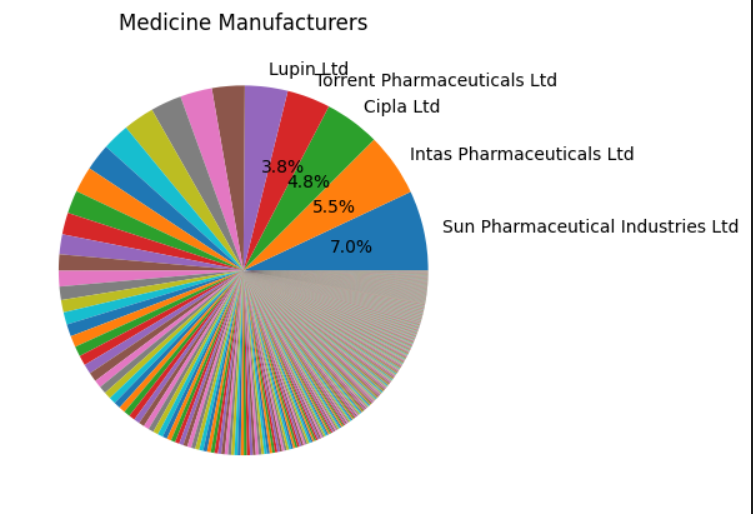
\includegraphics[width=\linewidth]{graphic1.png}
	\caption{Top Drug Manufacturers}
	\Description{Dataset Characterization \textit{\textbf{PRIMED}}'s data}
	\label{fig:topManufacturers}
  \end{figure}

\begin{figure}[H]
	\centering
	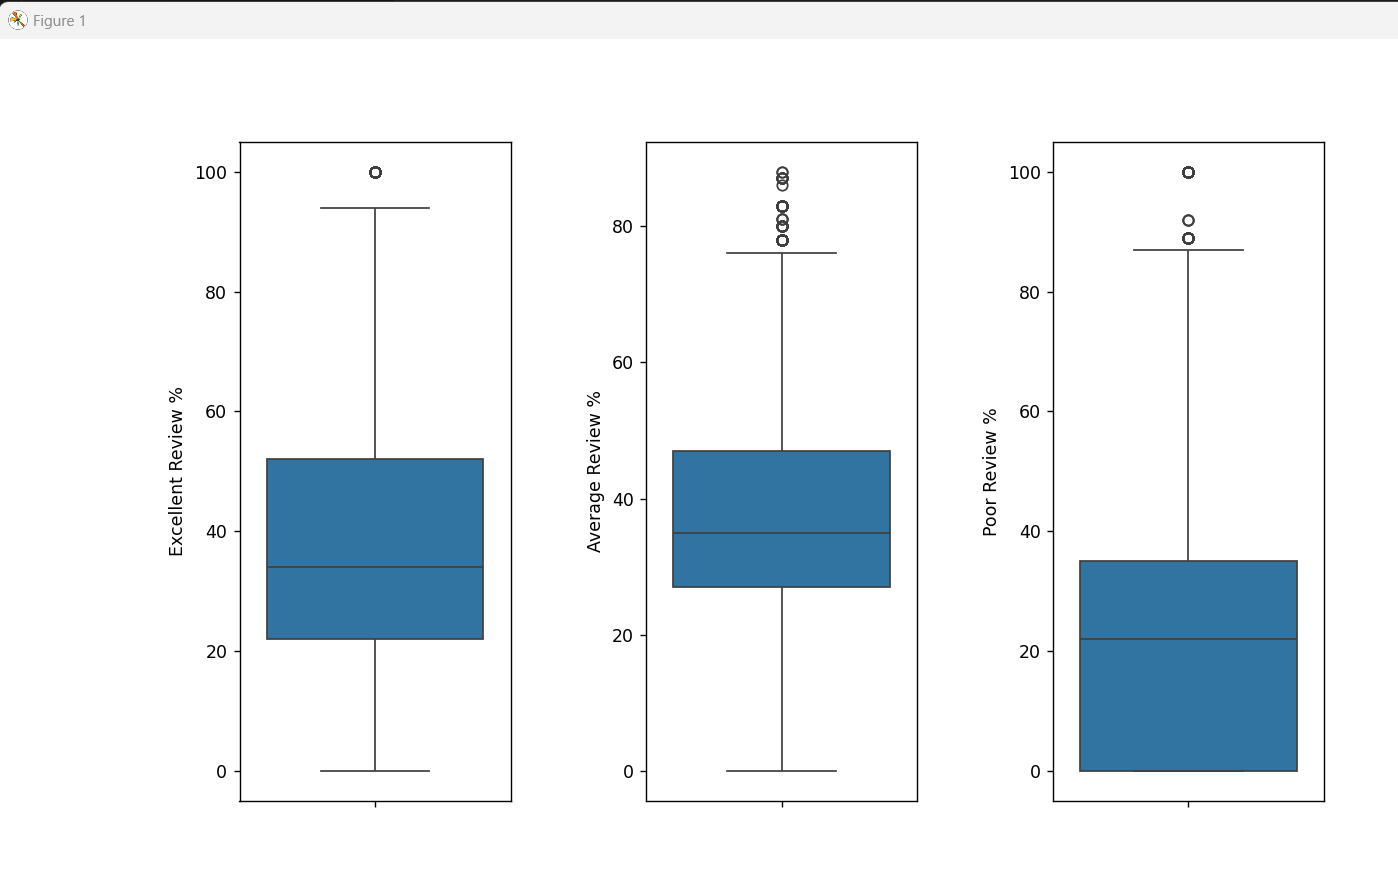
\includegraphics[width=\linewidth]{graphic2.png}
	\caption{Distribution of Reviews}
	\Description{Dataset Characterization \textit{\textbf{PRIMED}}'s data}
	\label{fig:reviewDistribution}
  \end{figure}

\begin{figure}[H]
	\centering
	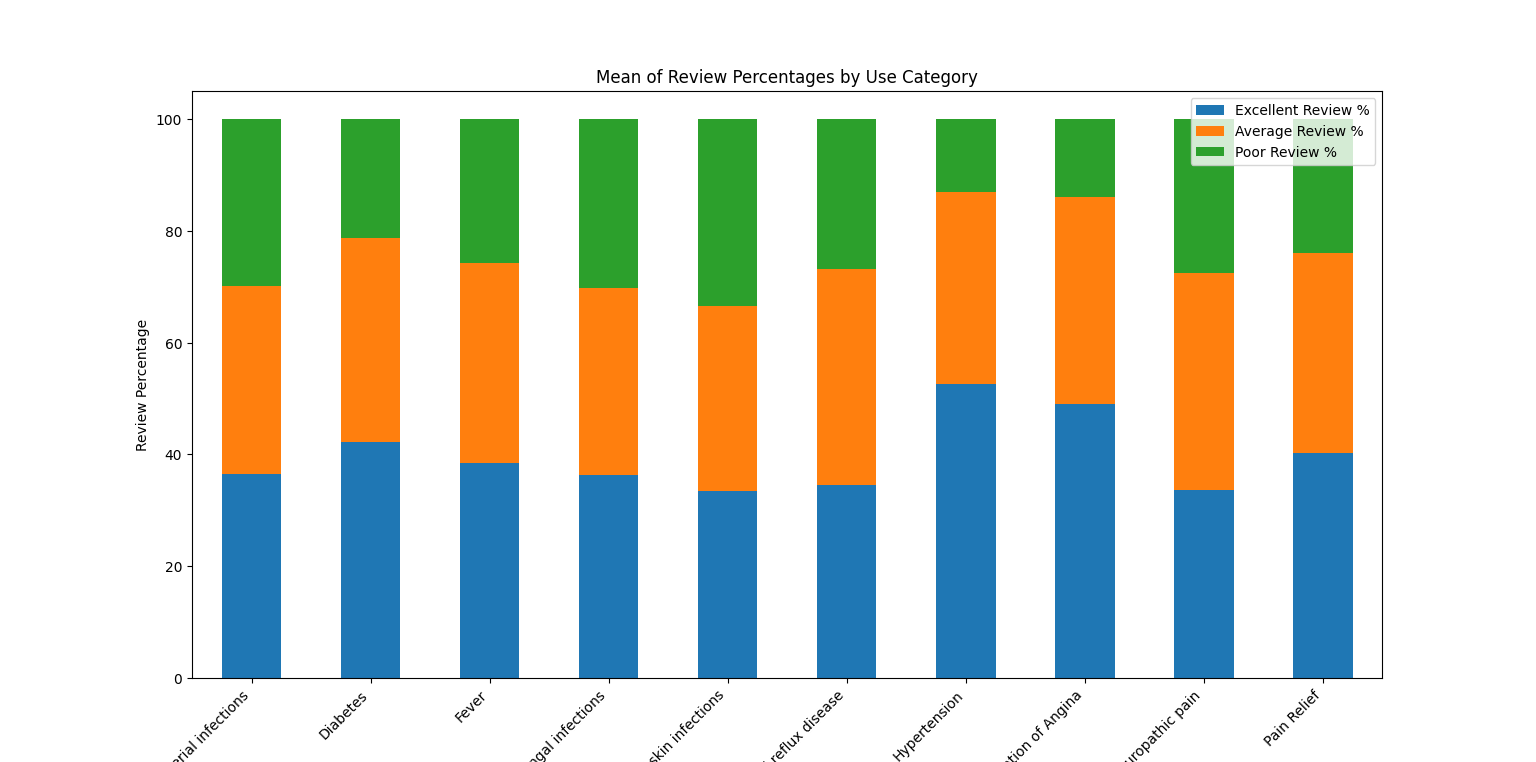
\includegraphics[width=\linewidth]{graphic3.png}
	\caption{Mean of Reviews Percentages by Uses}
	\Description{Dataset Characterization \textit{\textbf{PRIMED}}'s data}
	\label{fig:reviewPercMean}
  \end{figure}

\begin{figure}[H]
	\centering
	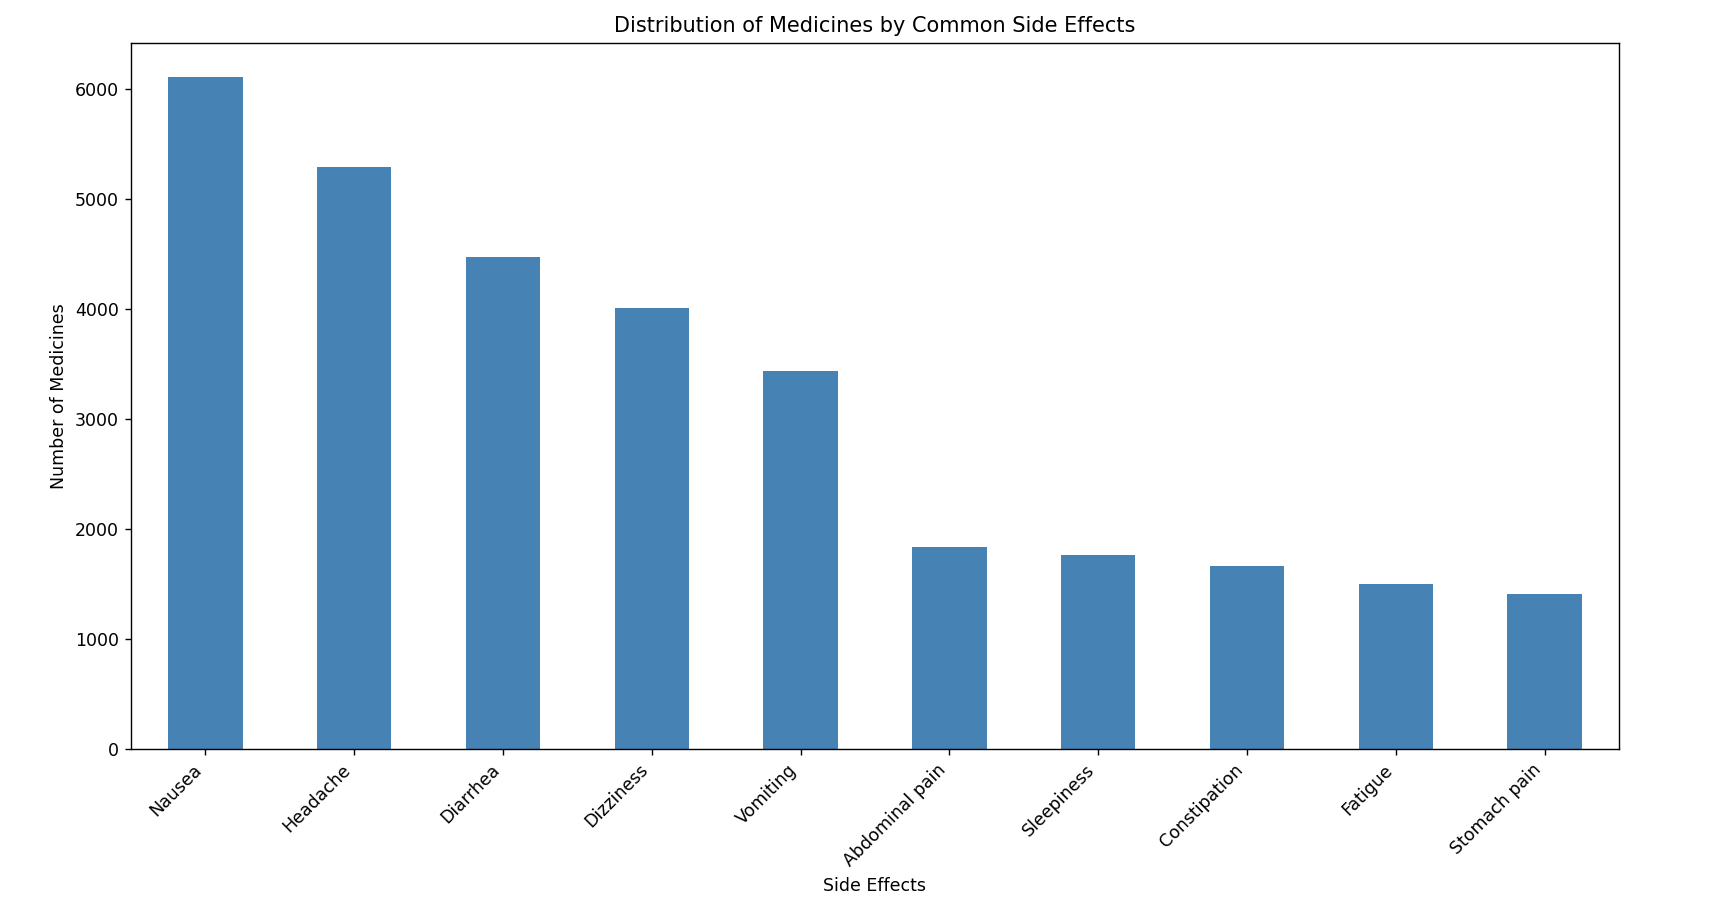
\includegraphics[width=\linewidth]{graphic4.png}
	\caption{Distribution of Side Effects}
	\Description{Dataset Characterization \textit{\textbf{PRIMED}}'s data}
	\label{fig:sideEffectsDistribution}
  \end{figure}

\begin{figure}[H]
	\centering
	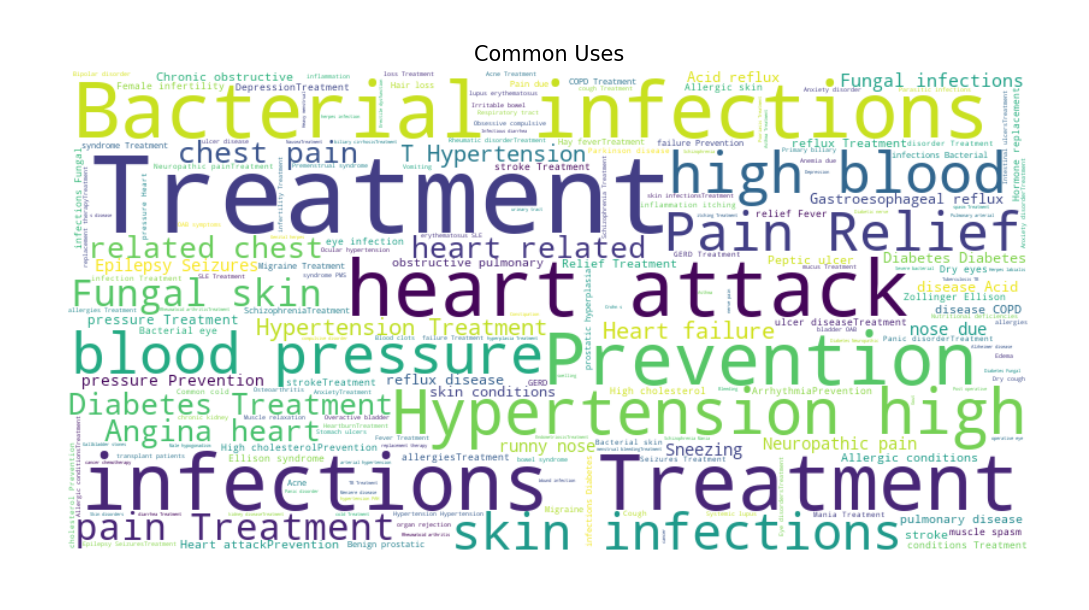
\includegraphics[width=\linewidth]{graphic5.png}
	\caption{Common Uses Word Cloud}
	\Description{Dataset Characterization \textit{\textbf{PRIMED}}'s data}
	\label{fig:commonUses}
  \end{figure} 

\begin{figure}[H]
	\centering
	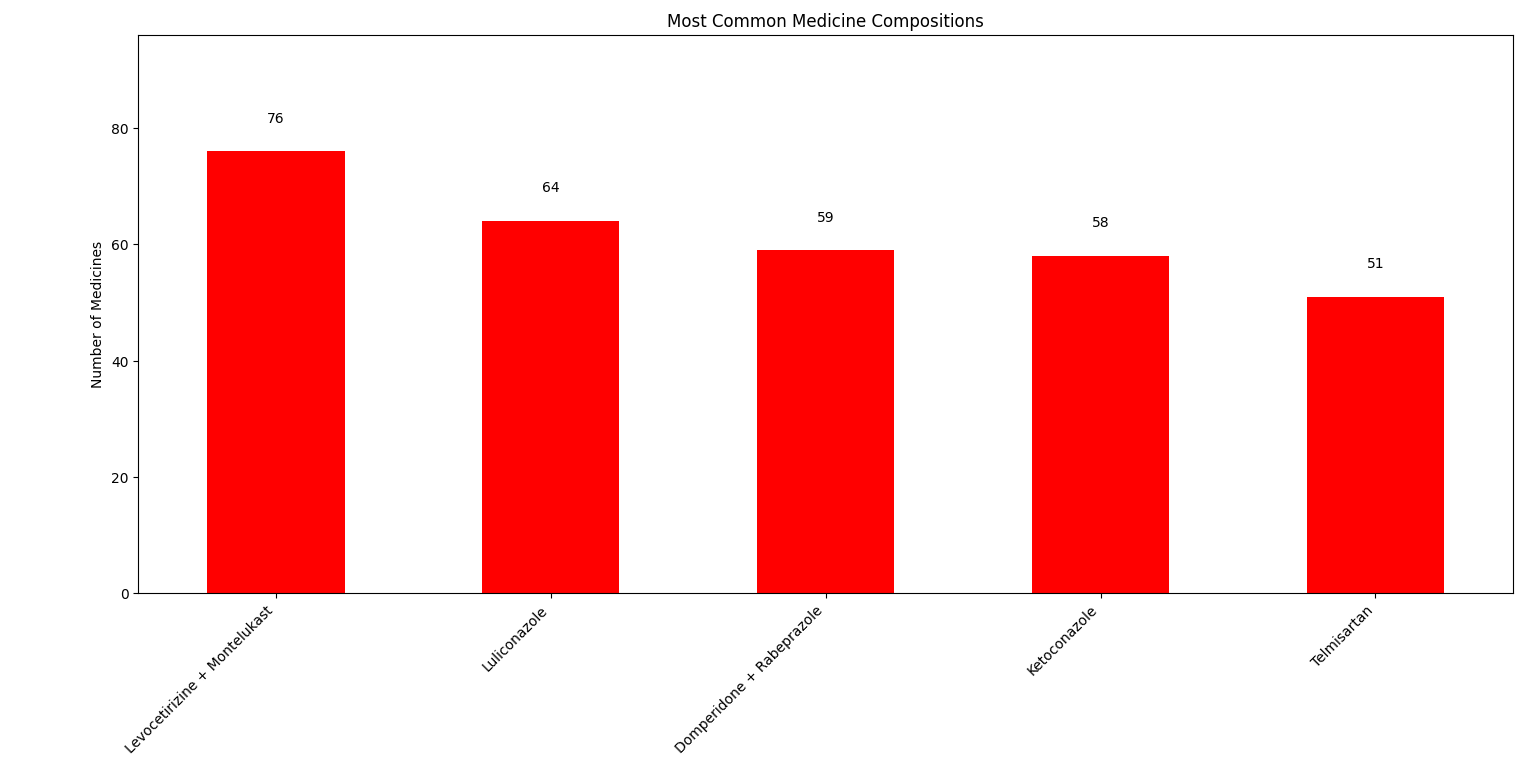
\includegraphics[width=\linewidth]{graphic6.png}
	\caption{Most Common Drug Compositions}
	\Description{Dataset Characterization \textit{\textbf{PRIMED}}'s data}
	\label{fig:commonDrugCompositions}
  \end{figure}   

\begin{figure}[H]
	\centering
	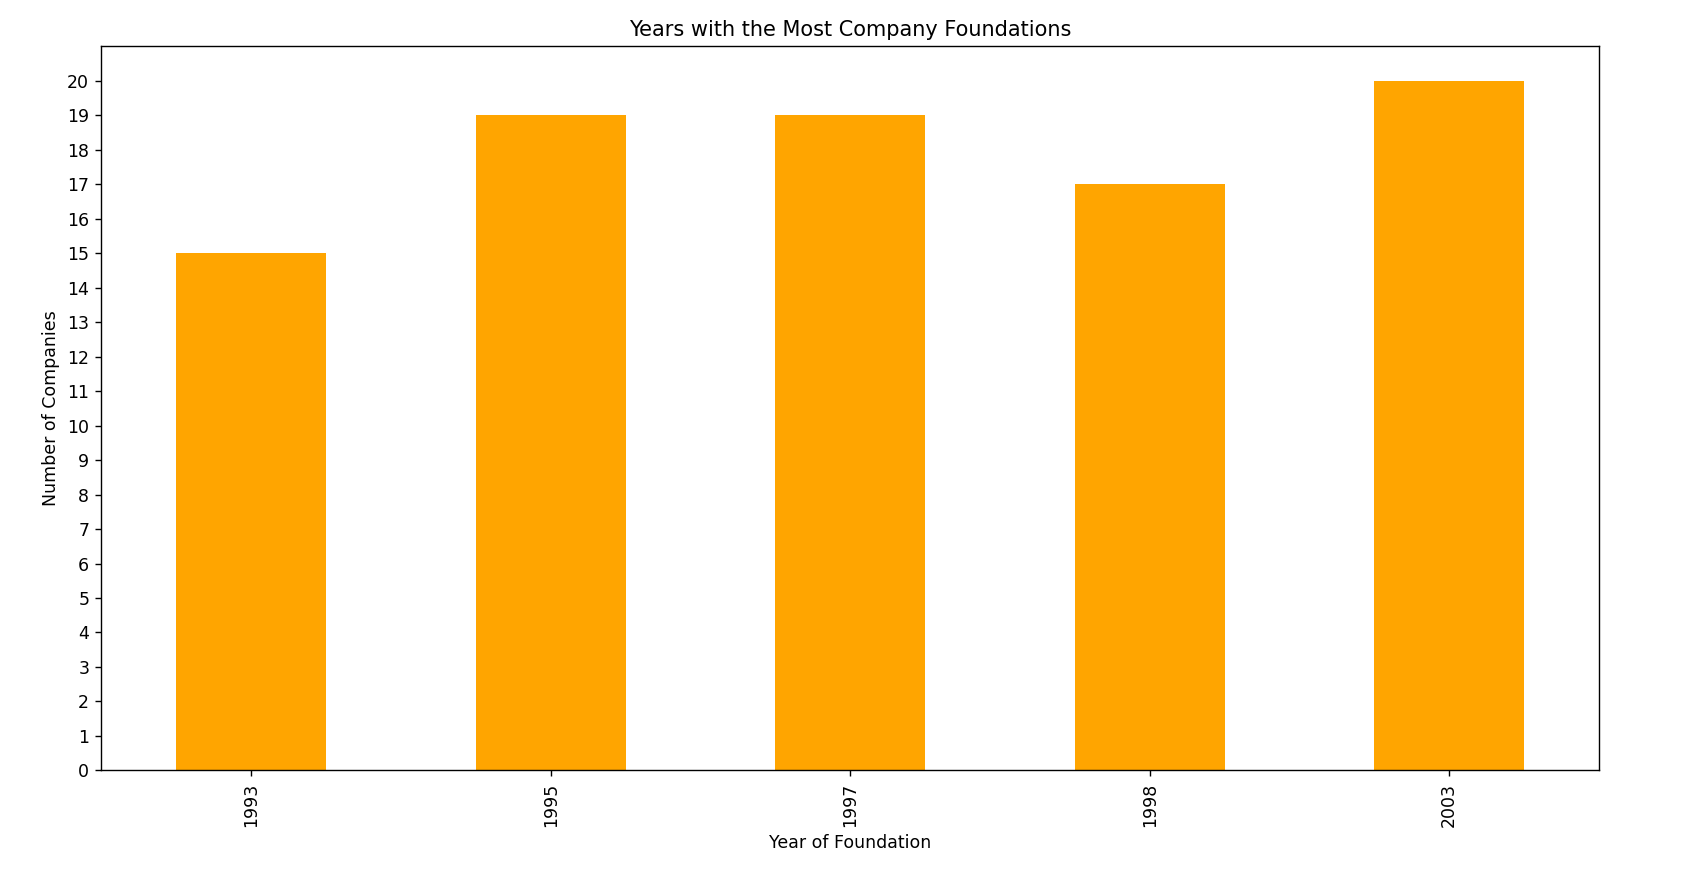
\includegraphics[width=\linewidth]{graphic7.png}
	\caption{Years with the Most Companies Foundations}
	\Description{Dataset Characterization \textit{\textbf{PRIMED}}'s data}
	\label{fig:companyYears}
  \end{figure}

\begin{figure}[H]
	\centering
	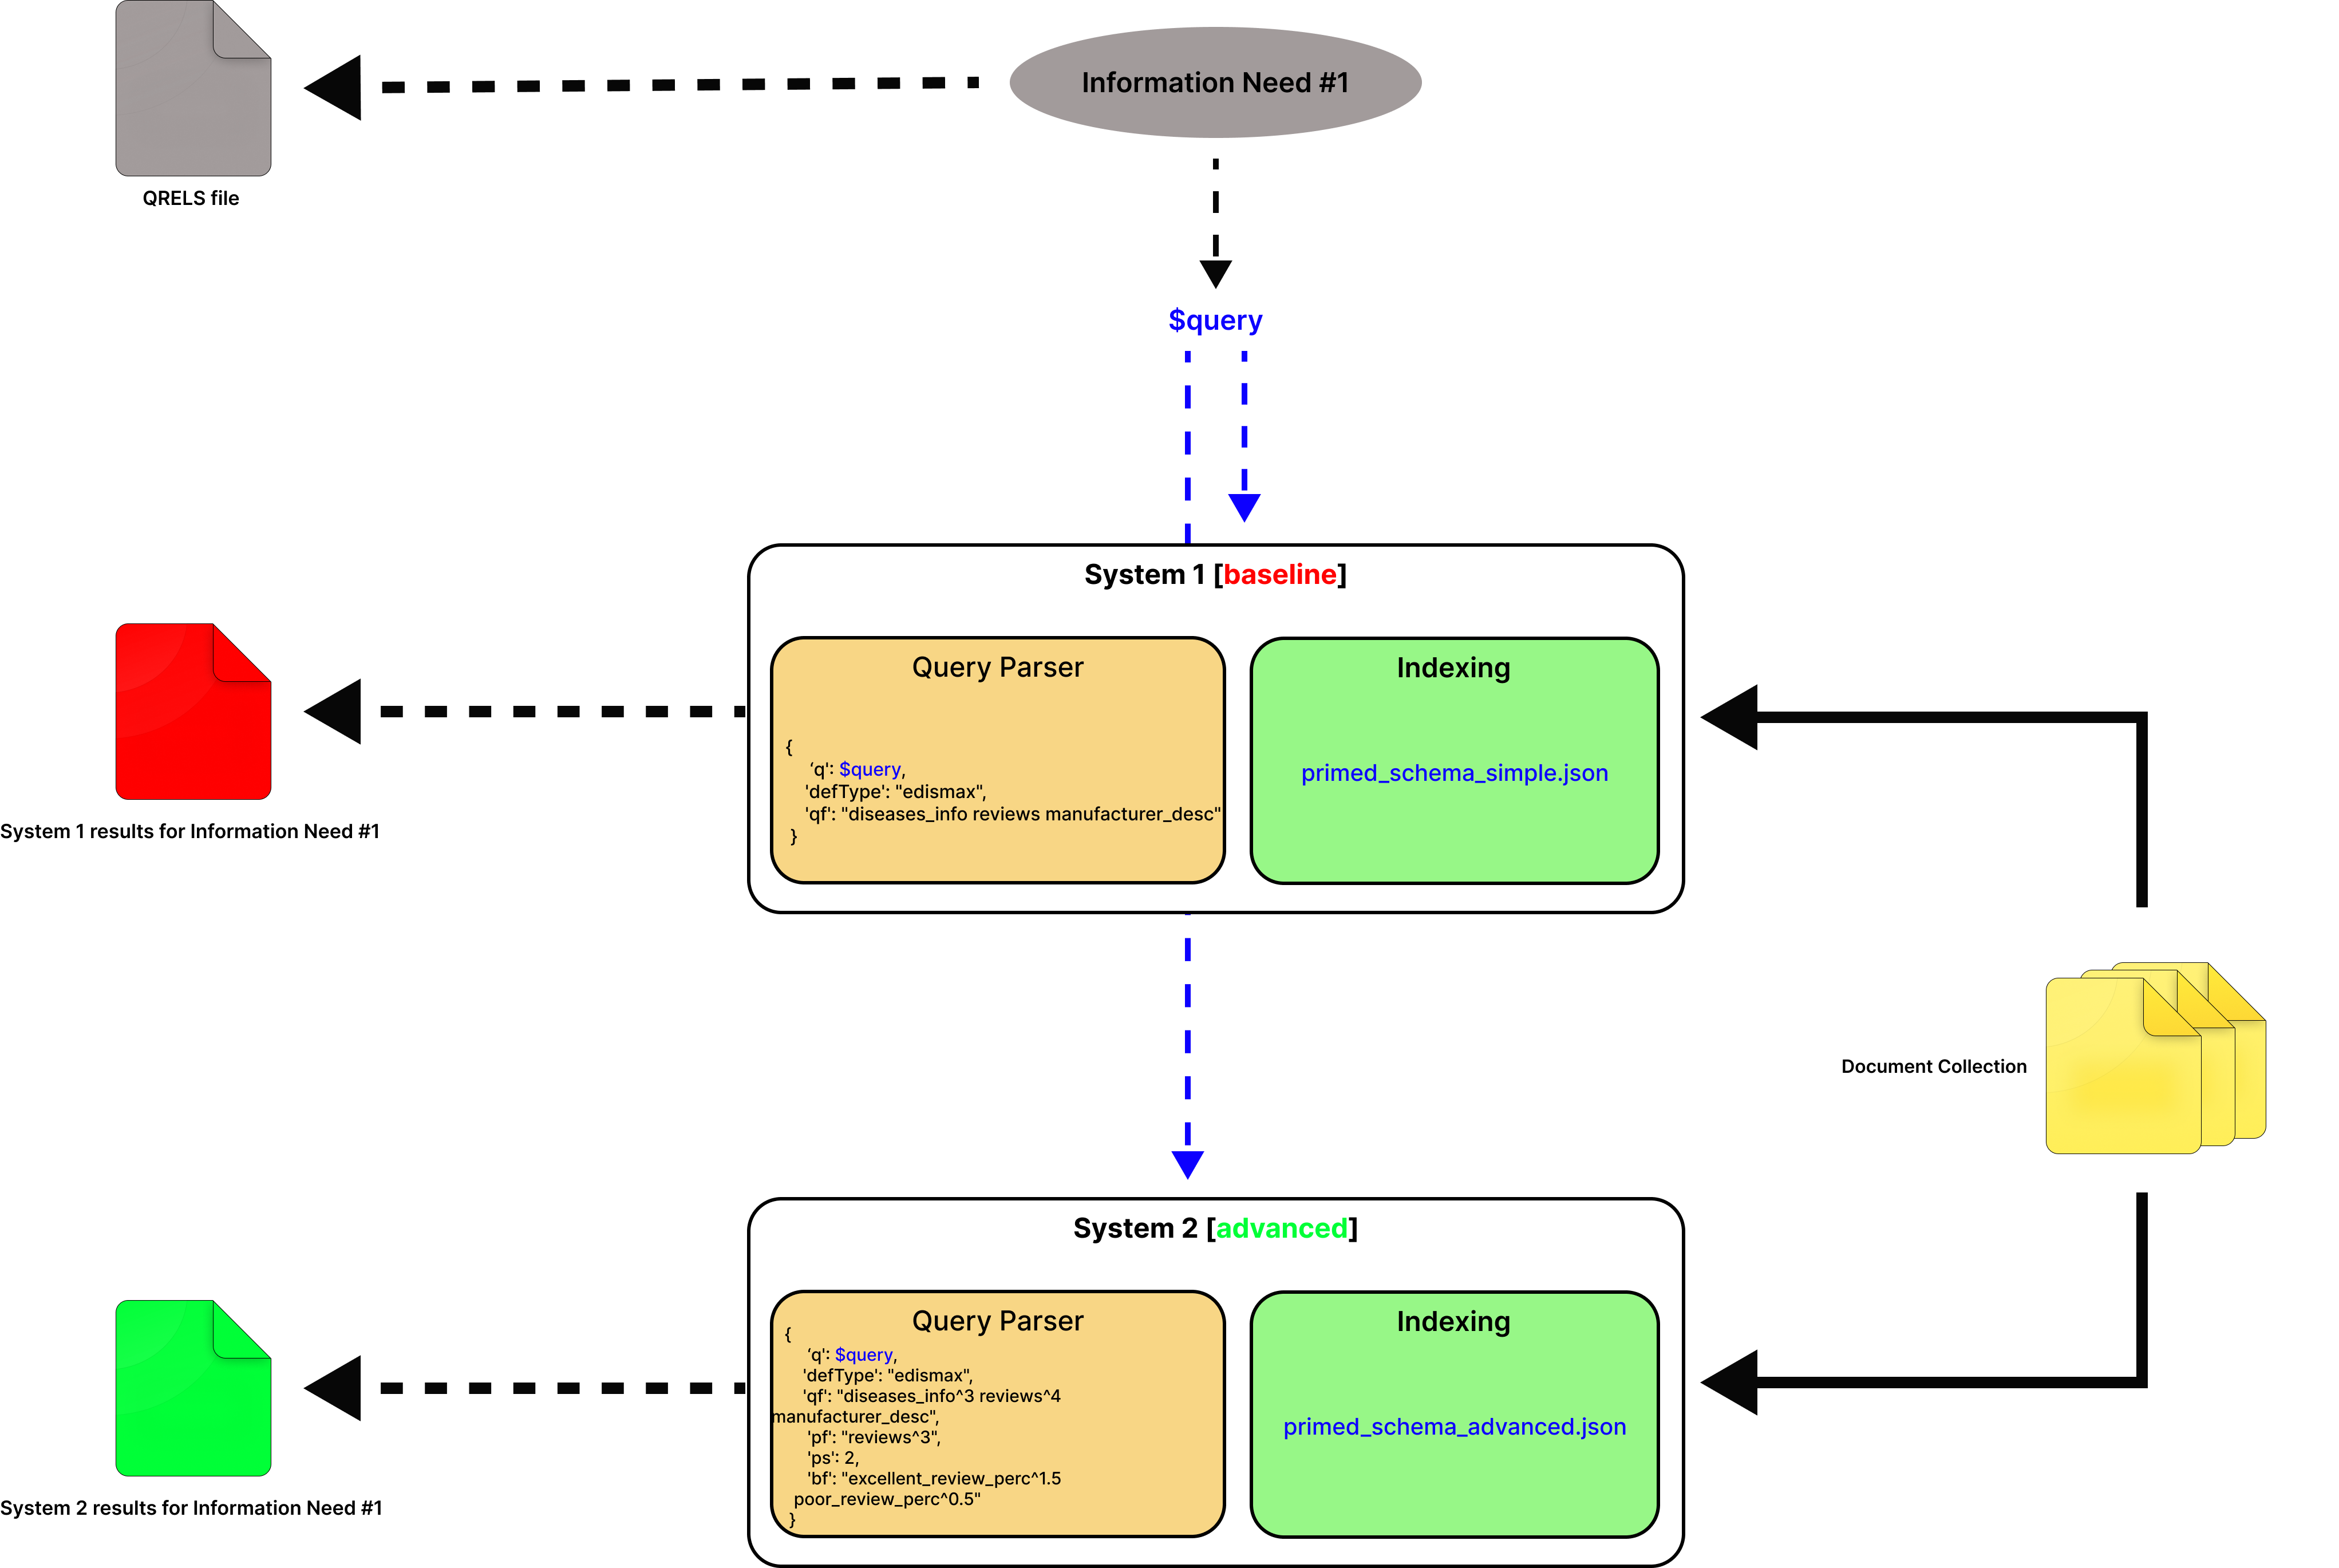
\includegraphics[width=\linewidth]{system_arch.png}
	\caption{System Architecture}
	\Description{\textit{\textbf{PRIMED}}'s Solr system architecture}
	\label{fig:sysArchitecture}
  \end{figure}
  
\begin{figure}[H]
  \centering
  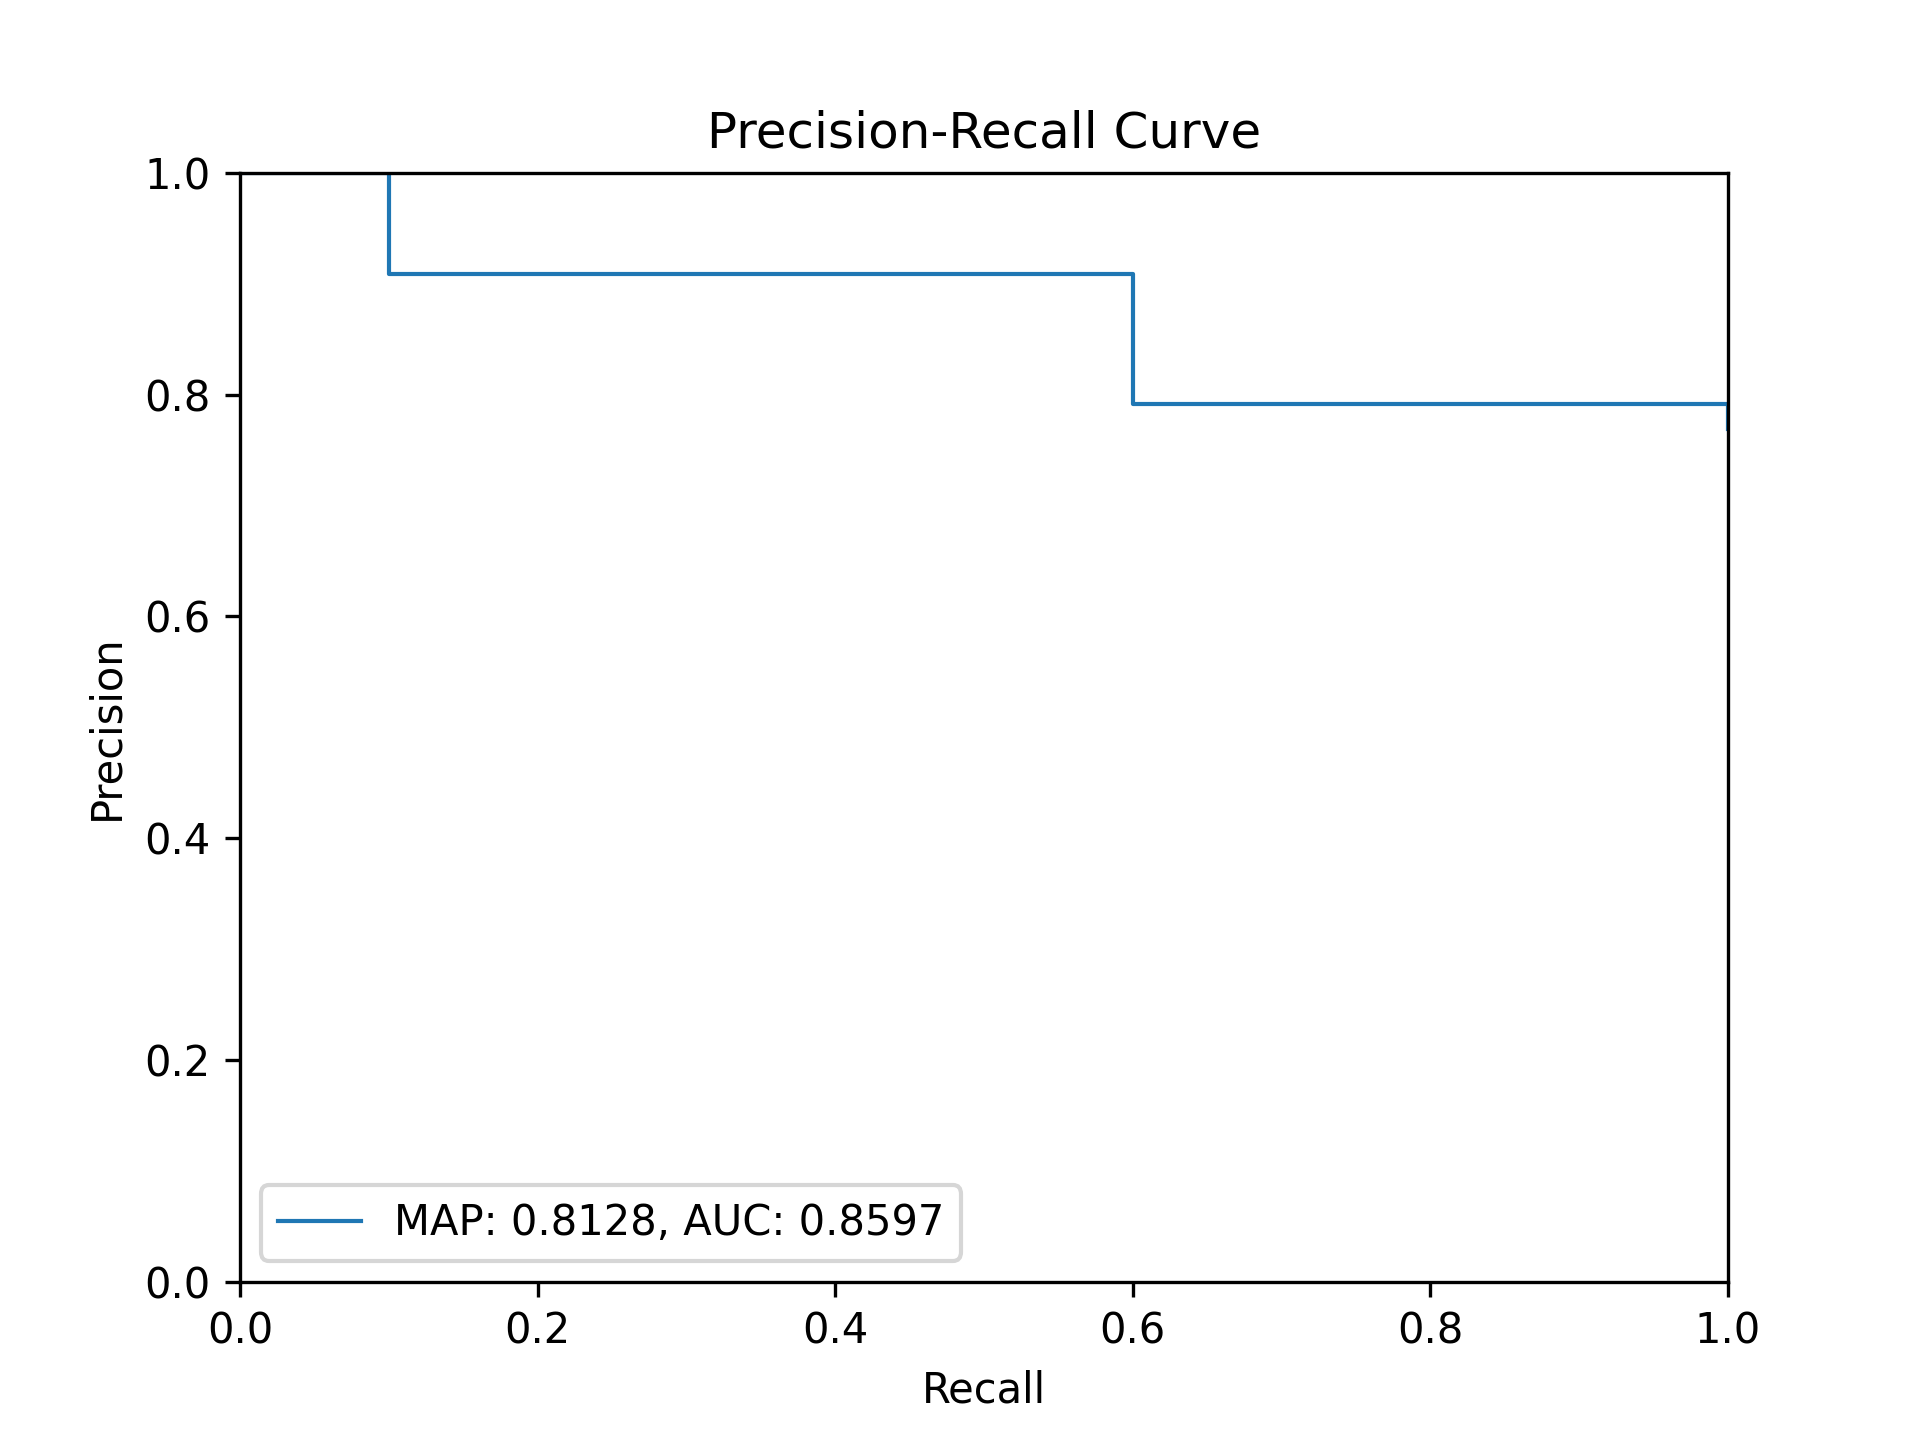
\includegraphics[width=\linewidth]{precision_recal_simple_1.png}
  \caption{Q1 P-R Curve -> Baseline System}
  \Description{Q1 P-R Curve -> Baseline System}
  \label{fig:precisionRecalSimple1}
\end{figure}

\begin{figure}[H]
  \centering
  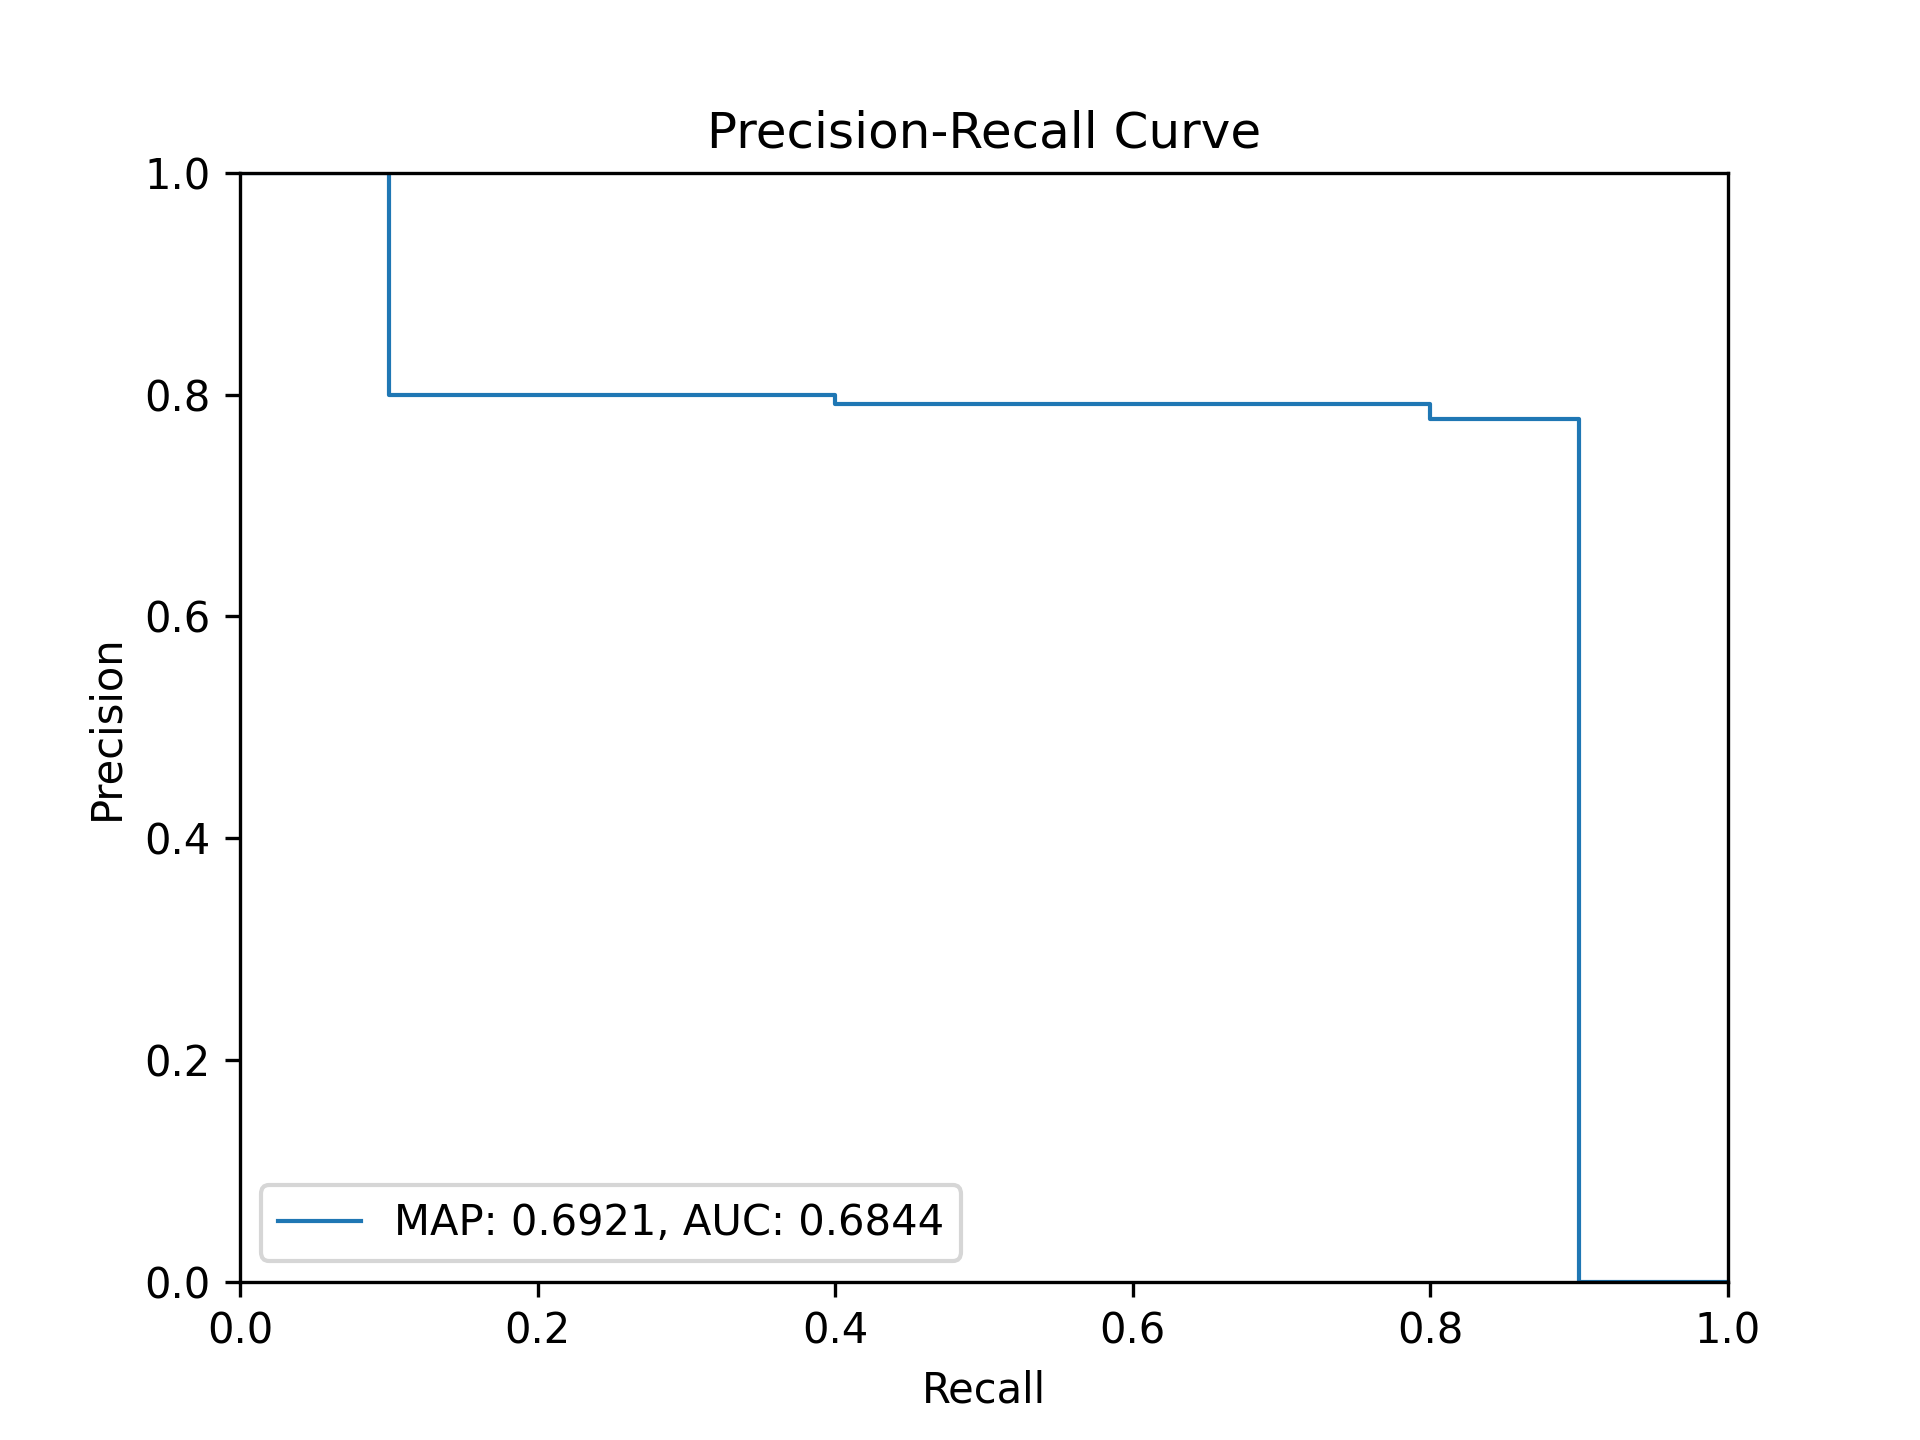
\includegraphics[width=\linewidth]{precision_recal_simple_2.png}
  \caption{Q2 P-R Curve -> Baseline System}
  \Description{Q2 P-R Curve -> Baseline System}
  \label{fig:precisionRecalSimple2}
\end{figure}
  
\begin{figure}[H]
	\centering
	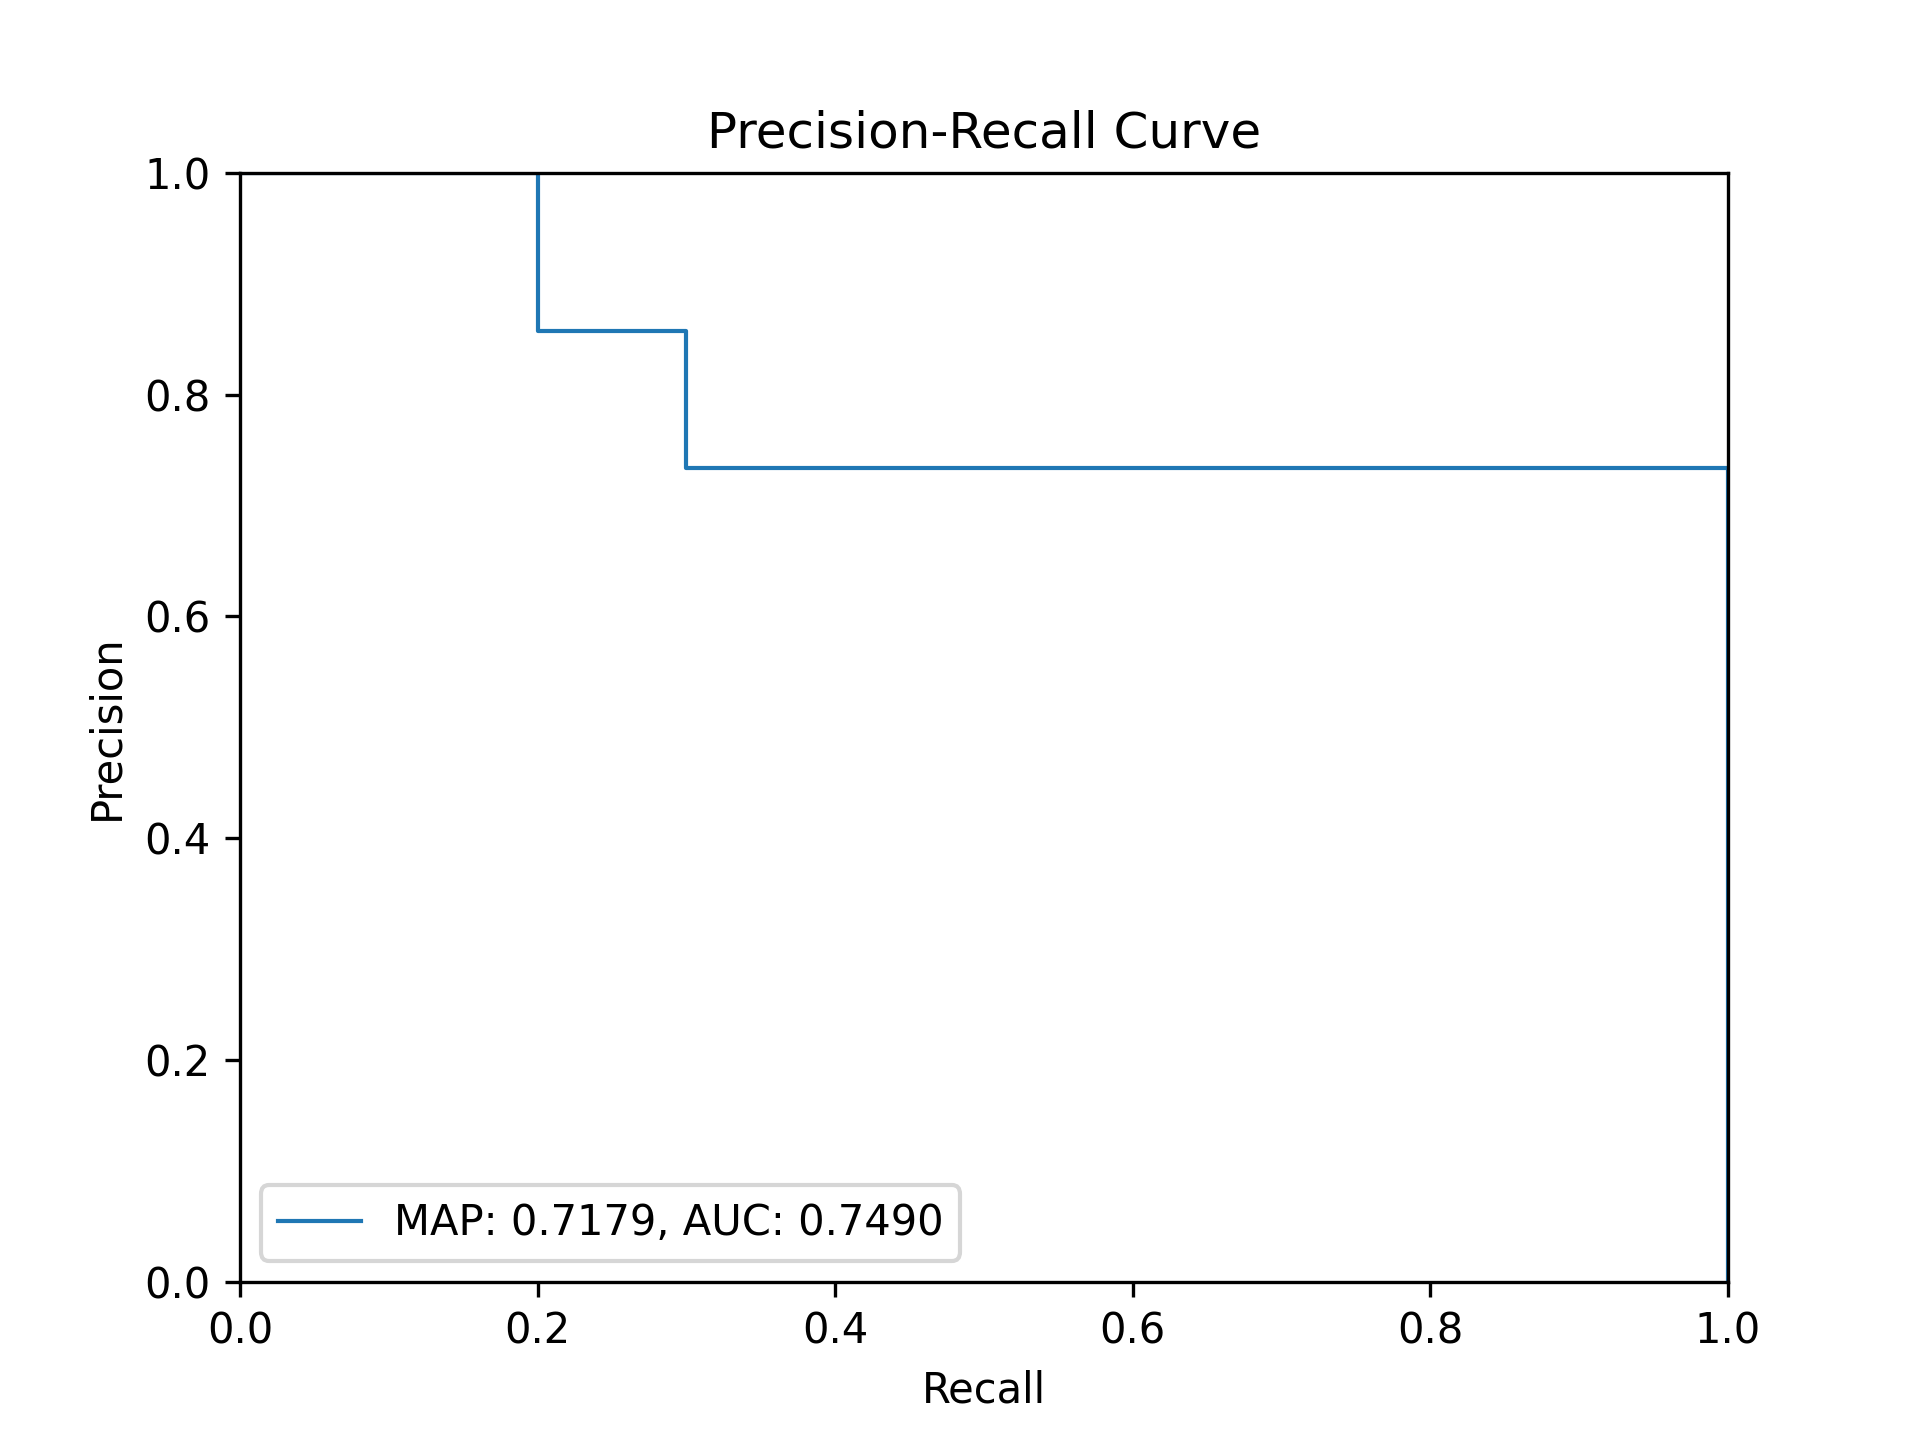
\includegraphics[width=\linewidth]{precision_recal_simple_3.png}
	\caption{Q3 P-R Curve -> Baseline System}
	\Description{Q3 P-R Curve -> Baseline System}
	\label{fig:precisionRecalSimple3}
\end{figure}

\begin{figure}[H]
  \centering
  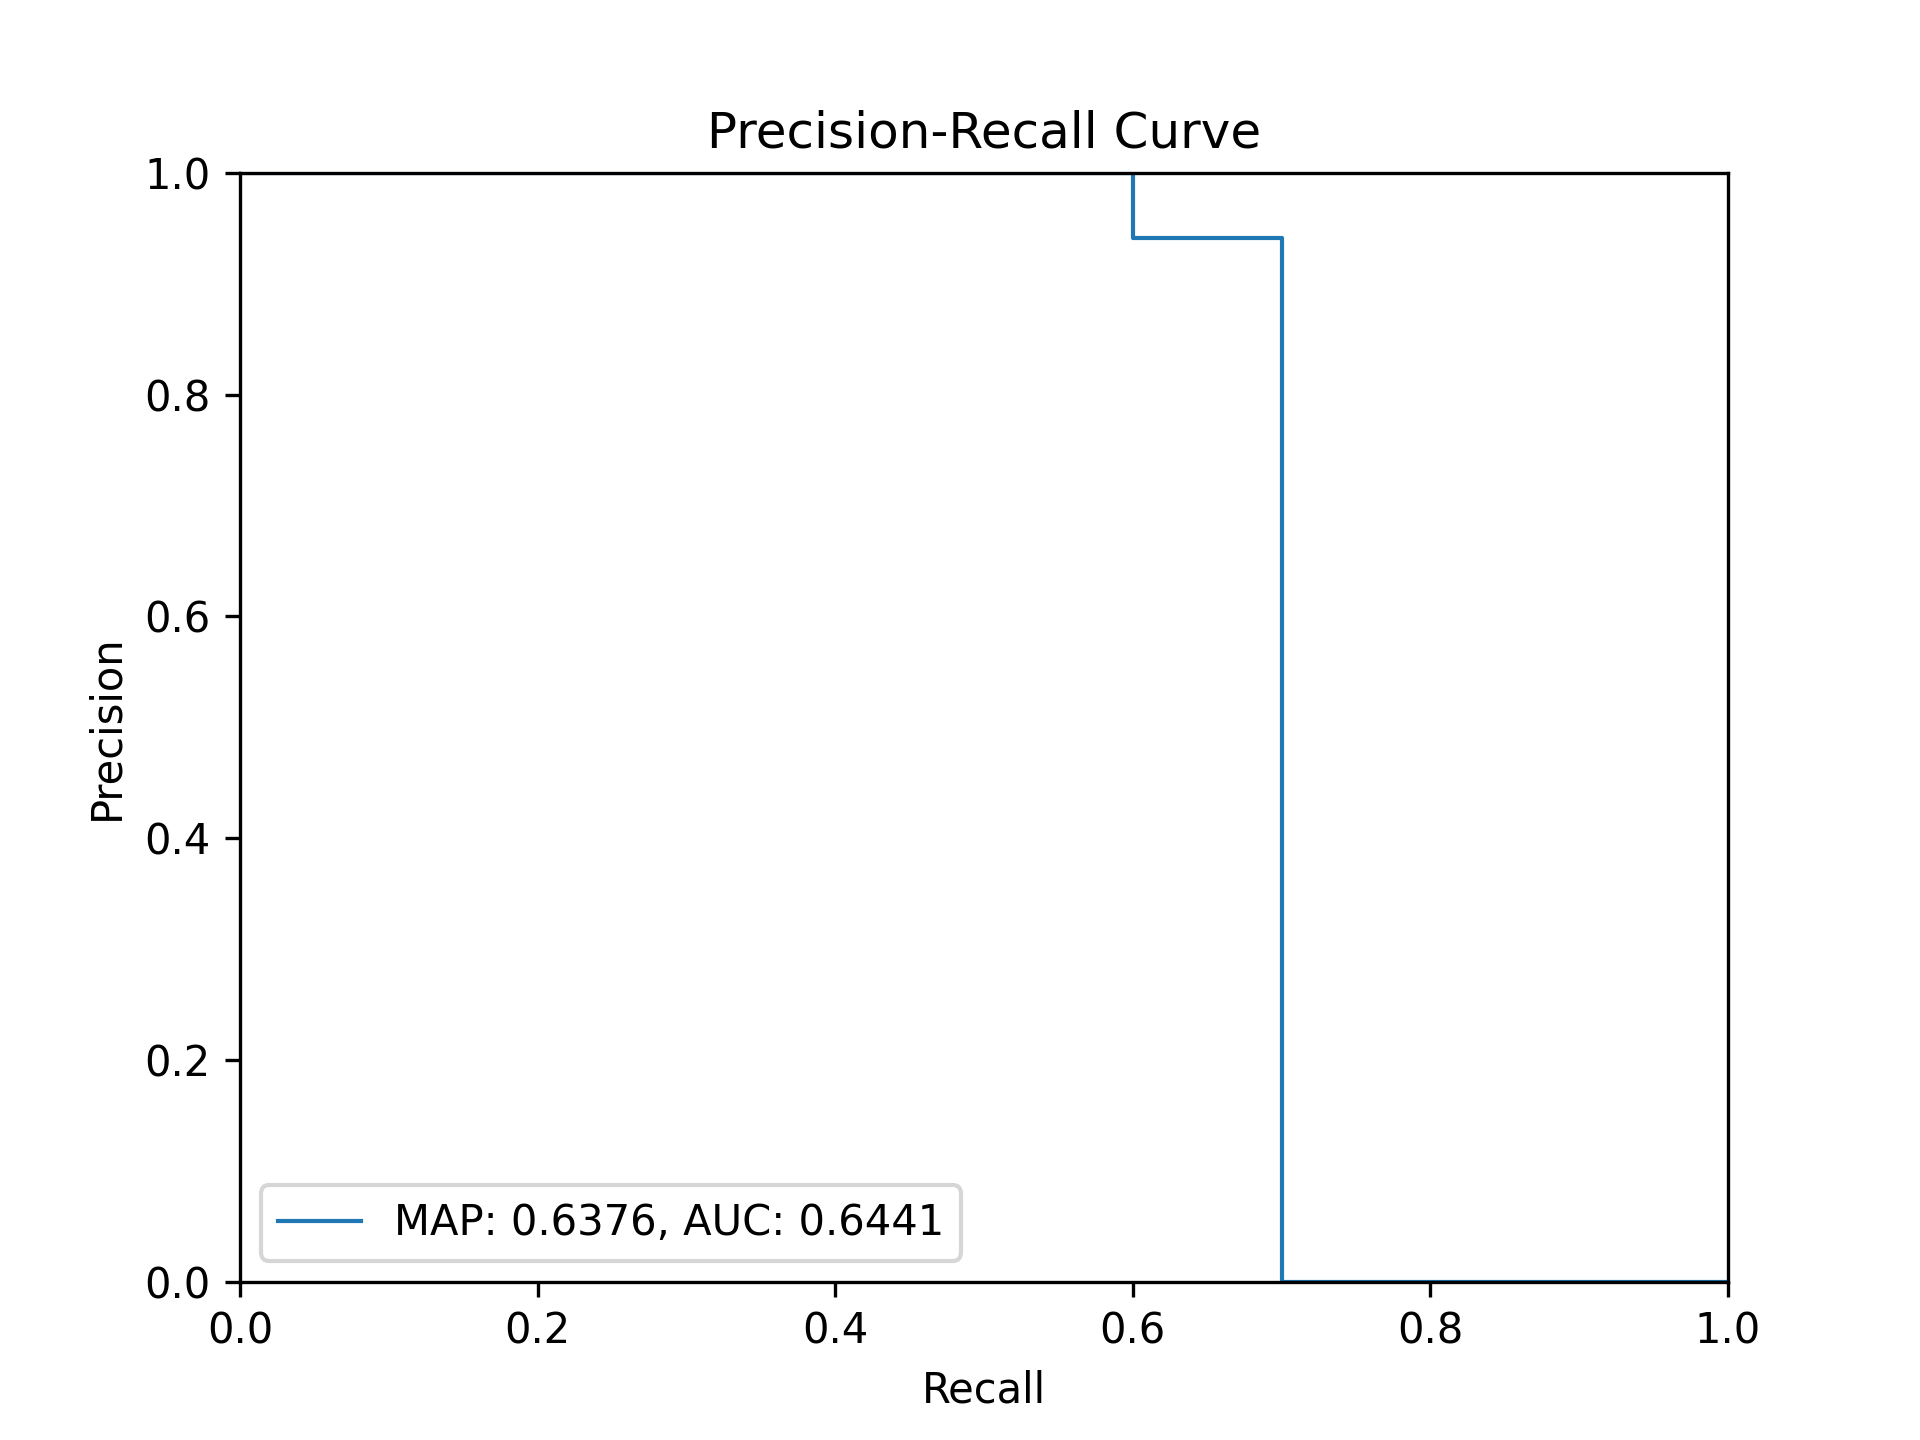
\includegraphics[width=\linewidth]{precision_recal_simple_4.png}
  \caption{Q4 P-R Curve -> Baseline System}
  \Description{Q4 P-R Curve -> Baseline System}
  \label{fig:precisionRecalSimple4}
\end{figure}

%%
%% The next two lines define the bibliography style to be used, and
%% the bibliography file.
%%\bibliographystyle{ACM-Reference-Format}
\bibliographystyle{unsrt}
\bibliography{sample-base}


%%
%% If your work has an appendix, this is the place to put it.
%%\appendix

\end{document}
\endinput
%%
%% End of file `sample-sigconf-authordraft.tex'.
